% MURI review talk, 2026-08-21 (20 min) --- cascaded chi2:chi2 -> chi3 metasurfaces
% Build: pdflatex (twice). All numbers follow the post-2026-05/07 canonical values.
\documentclass[aspectratio=169,10pt]{beamer}

\usetheme{metropolis}
\metroset{block=fill, numbering=fraction, progressbar=frametitle, sectionpage=progressbar}

\usepackage[T1]{fontenc}
\usepackage{amsmath,amssymb,bm}
\usepackage{booktabs}
\usepackage{graphicx}
\usepackage{xcolor}
\usepackage{tikz}
\usetikzlibrary{arrows.meta}

\graphicspath{{muri_figs/}%
              {../cascaded_chi3/figures/}%
              {../cascaded_chi3/figures/combined/}%
              {../cascaded_chi3/figures/design6/}%
              {../cascaded_chi3/figures/samples/}}

% shorthands (same conventions as the notes)
\newcommand{\chitwo}{\chi^{(2)}}
\newcommand{\chithree}{\chi^{(3)}}
\newcommand{\chicasc}{\chi^{(3)}_{\mathrm{casc}}}
\newcommand{\chinat}{\chi^{(3)}_{\mathrm{native}}}
\newcommand{\Dom}{\Delta\omega}
\newcommand{\gtwo}{\gamma_2}
\newcommand{\gone}{\gamma_1}
\definecolor{good}{HTML}{2ca02c}
\definecolor{bad}{HTML}{d62728}
\definecolor{d6}{HTML}{9467bd}
\definecolor{up}{HTML}{1f77b4}
\definecolor{dn}{HTML}{9467bd}
\definecolor{sh}{HTML}{d62728}
\newcommand{\yes}{\textcolor{good}{\textbf{yes}}}
\newcommand{\no}{\textcolor{bad}{\textbf{no}}}
\setbeamerfont{footnote}{size=\tiny}

\title{A synthesised Kerr nonlinearity: cascaded $\chitwo{:}\chitwo$ \\ in LiNbO$_3$ metasurfaces}
\author{Nikita Nefedkin\inst{1} \and Sedigheh Esfahani\inst{1} \and
        Jacob B. Khurgin\inst{2} \and Andrea Al\`u\inst{1}}
\institute{\inst{1}Photonics Initiative, Advanced Science Research Center,
           City University of New York \\
           \inst{2}Department of Electrical and Computer Engineering,
           Johns Hopkins University \\[6pt]
           % 
\includegraphics[height=0.42cm]{muri_logos}
       }
\date{MURI Meeting --- August 21, 2026}

\begin{document}

\maketitle

% ===============================================================
\section{Motivation and idea}

% ---------------------------------------------------------------
\begin{frame}{Why we want a larger Kerr response}
  \textbf{Kerr ($\chithree$) underpins all-optical photonics:} phase control,
  switching, four-wave mixing, frequency combs, all driven by a single pump.
  \vspace{4pt}
  \begin{columns}[T]
    \begin{column}{0.56\linewidth}
      \footnotesize
      \begin{table}
      \begin{tabular}{@{}lccl@{}}
        \toprule
        Host & $|\chitwo|$ & $|\chithree|$ [m$^2$/V$^2$] & limitation \\
        \midrule
        SiO$_2$   & 0 & $\sim\!3\times10^{-22}$ & very weak Kerr \\
        \textbf{LiNbO$_3$} & \textbf{50 pm/V} & $\bm{\sim\!2\times10^{-21}}$ & \textbf{weak Kerr} \\
        Si        & 0 & $\sim\!10^{-19}$ & TPA + free carriers \\
        AlGaAs    & 100 pm/V & $\sim\!10^{-18}$ & band-edge loss, heat \\
        \bottomrule
      \end{tabular}
      \end{table}
    \end{column}
    \begin{column}{0.4\linewidth}
      \small
      Materials with a \emph{large} Kerr pay for it in loss and heat, while the
      cleanest $\chitwo$ platform, LiNbO$_3$, has a Kerr $\sim\!100\times$
      \emph{weaker} than silicon.
      \vspace{3pt}

      The same trade extends to the III--V semiconductors in our program, with
      engineered $\chitwo$ up to $\sim$10$\times$ LiNbO$_3$'s.
      \\[1pt]
      {\tiny\color{gray} Ramesh \emph{et al.}, Optica, in press; arXiv:2602.23246}
    \end{column}
  \end{columns}
  \vspace{6pt}
  \begin{alertblock}{The question}
    Can we \emph{synthesise} a large, controllable $\chithree$ from a strong
    $\chitwo$, instead of accepting a weak native Kerr?
  \end{alertblock}
\end{frame}

% ---------------------------------------------------------------
\begin{frame}{Cascaded nonlinearities: prior work and what is new here}
  \textbf{Two sequential $\chitwo$ processes}, SHG followed by DFG: the round trip acts
  as an effective Kerr response.
  \vspace{2pt}
  \small
  \begin{itemize}\setlength\itemsep{2pt}
    \item \textbf{1967}: predicted, as a nonlinear phase from phase-mismatched SHG.
          \hfill {\tiny\color{gray} Ostrovskii, JETP Lett.\ \textbf{5}, 272}
    \item \textbf{1992}: measured, as a Z-scan through the phase-match angle in KTP; the
          nonlinear refraction \emph{changes sign} at $\Delta k = 0$.
          \hfill {\tiny\color{gray} DeSalvo \emph{et al.}, Opt.\ Lett.\ \textbf{17}, 28}
    \item \textbf{1996--97}: reviewed; understood microscopically as a collective,
          virtual-SH effect. \\
          \mbox{}\hfill {\tiny\color{gray} Stegeman \emph{et al.}, Opt.\ Quantum Electron.\ \textbf{28}, 1691;\ \ Khurgin \emph{et al.}, JOSA B \textbf{14}, 1977}
    \item \textbf{2022}: cascading reaches metasurfaces, but for \emph{harmonic
          generation} (THG via SHG+SFG in GaAs), not for a Kerr response on the pump.
          \hfill {\tiny\color{gray} Gennaro \emph{et al.}, ACS Photonics \textbf{9}, 1026}
  \end{itemize}
  \vspace{4pt}
  \begin{block}{What is new here}
    In bulk, the cascade lever is the phase mismatch: $\chicasc \propto 1/\Delta k$.
    We replace it with a \textbf{resonant lever}, a high-$Q$, \emph{dark} resonance at the
    second harmonic: $\chicasc \propto Q_2/\Dom$, detuning-tunable, chip-scale,
    and CW-compatible.
  \end{block}
\end{frame}

% ---------------------------------------------------------------
\begin{frame}{Our starting point: quantum-engineered $\chitwo$ metasurfaces}
  \centering
  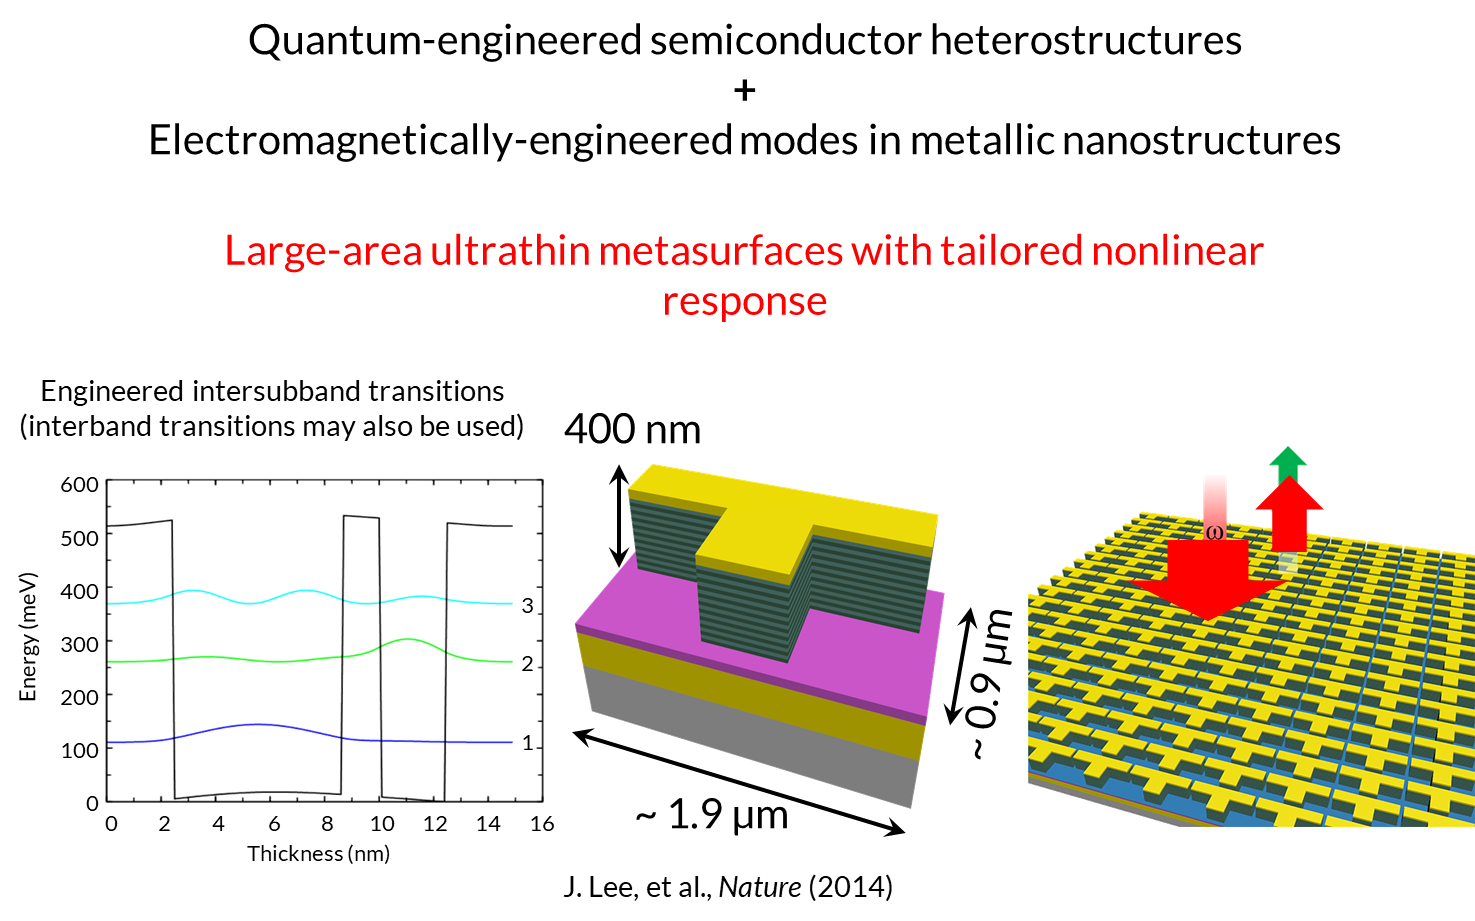
\includegraphics[width=0.6\linewidth]{group_mqw_metasurface}
  \vspace{2pt}

  \small
  Intersubband transitions in MQW heterostructures coupled to plasmonic modes:
  a 400-nm-thick metasurface with $|\chitwo| > 5\times10^{4}$\,pm/V at
  $\lambda\approx8\,\mu$m, SHG at normal incidence.
  \\[1pt]
  {\tiny\color{gray} J.~Lee \emph{et al.}, Nature \textbf{511}, 65 (2014)}
\end{frame}

% ---------------------------------------------------------------
\begin{frame}{From giant $\chitwo$ to full control of the second harmonic}
  \begin{columns}[T]
    \begin{column}{0.48\linewidth}
      \centering
      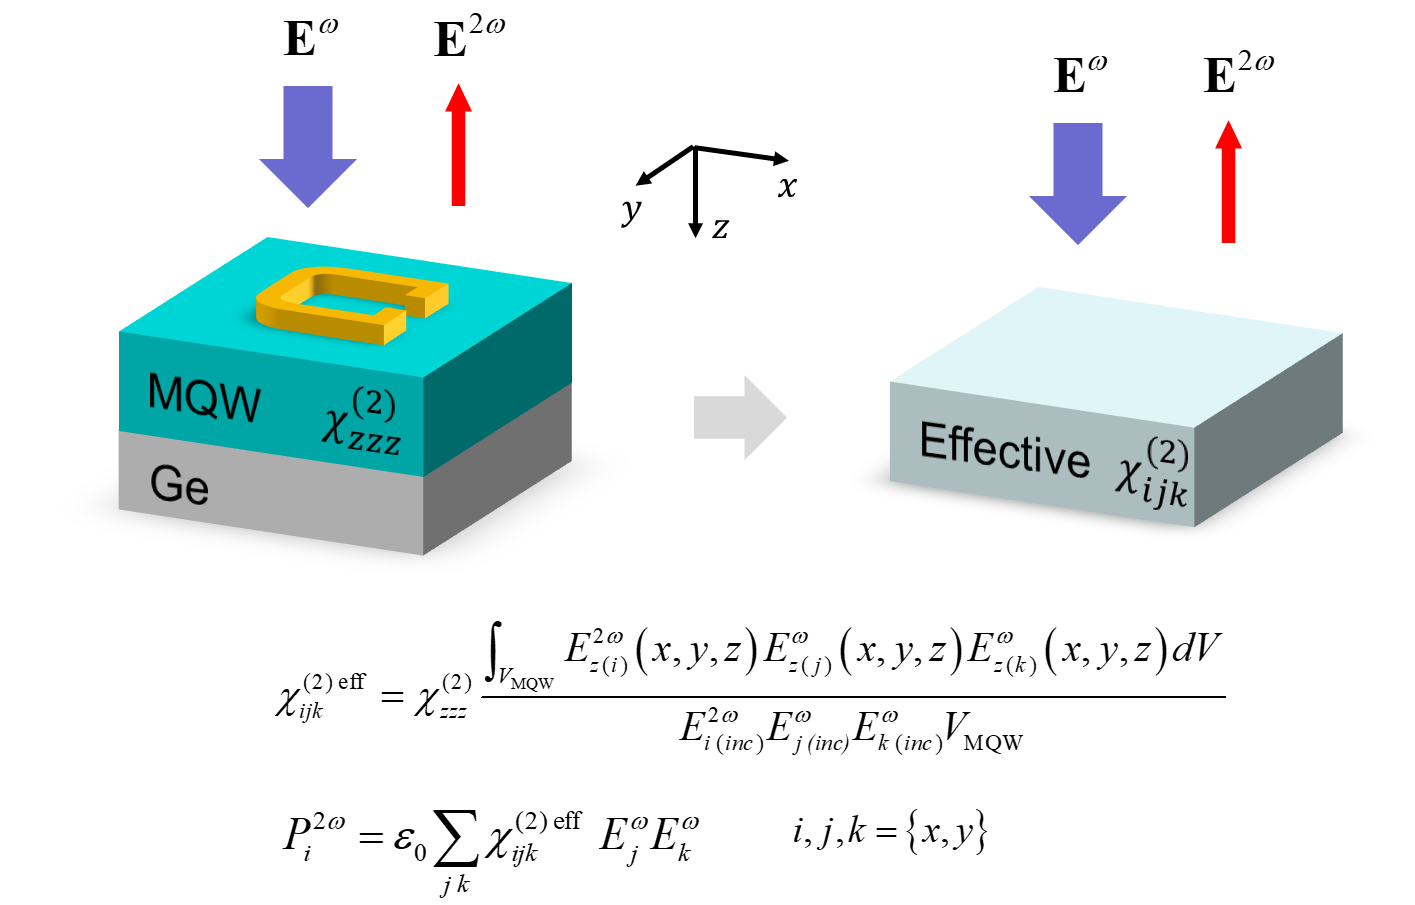
\includegraphics[width=0.82\linewidth]{group_effective_chi2}
    \end{column}
    \begin{column}{0.52\linewidth}
      \centering
      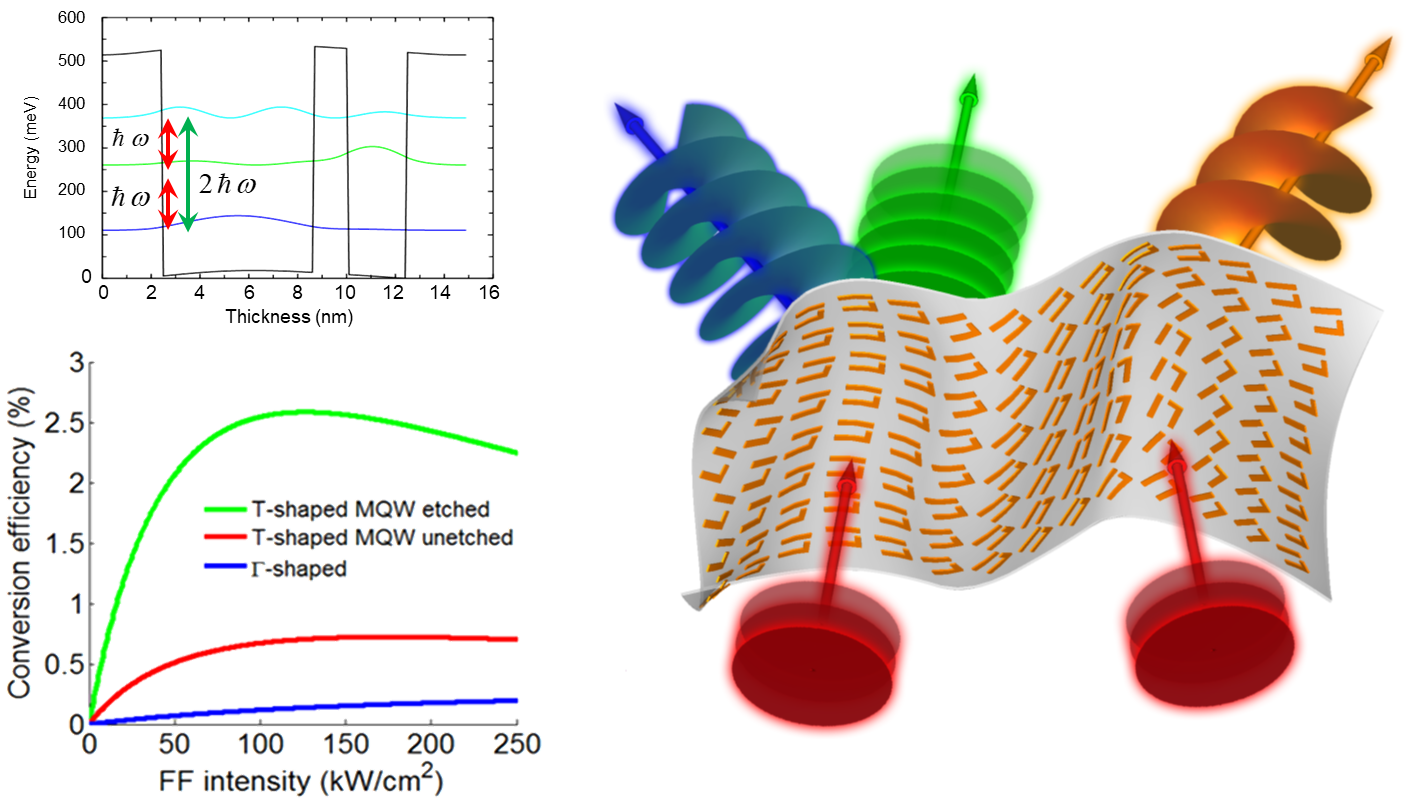
\includegraphics[width=0.84\linewidth]{group_flatland_nlo}
    \end{column}
  \end{columns}
  \vspace{2pt}
  \small
  Homogenised effective $\chi^{(2)}_{ijk}$ per meta-atom; SHG conversion up to
  $\sim$2.5\,\%, and gradient (Pancharatnam--Berry) phase control of the emitted
  second harmonic.
  \hfill {\tiny\color{gray} Tymchenko \emph{et al.}, PRL \textbf{115}, 207403 (2015);
  Nookala \emph{et al.}, Optica \textbf{3}, 283 (2016)}
  \vspace{1pt}
  \begin{block}{This project}
    Use the engineered $\chitwo$ \emph{twice}: convert it into an effective Kerr
    response on the pump.
  \end{block}
\end{frame}

% ---------------------------------------------------------------
\begin{frame}{Giant interband $\chitwo$ from coupled QWs}
  \centering
  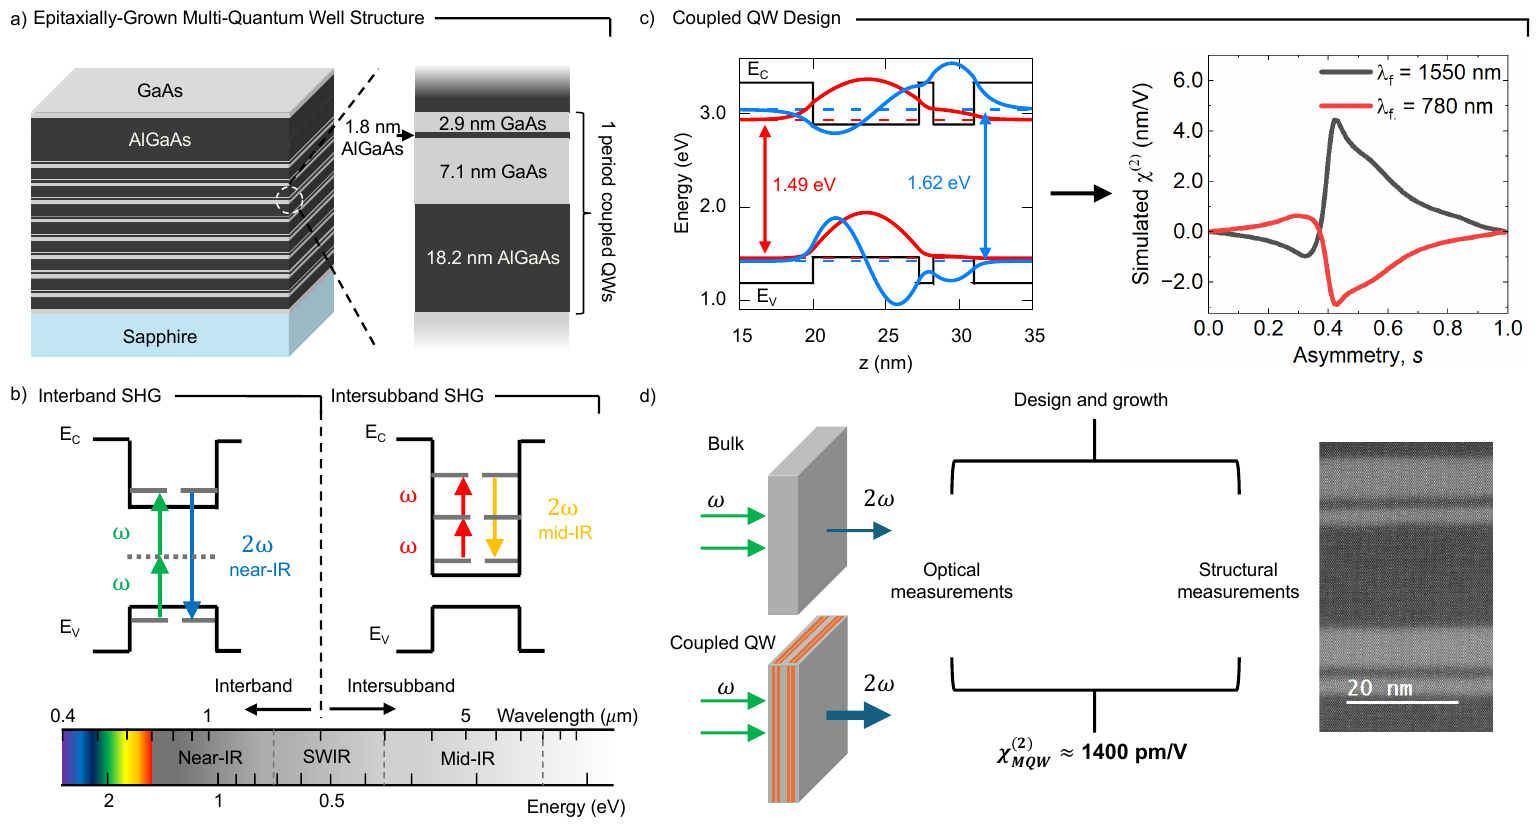
\includegraphics[width=0.64\linewidth]{cqw_fig1}
  \\[3pt]
  \small
  Asymmetric GaAs/AlGaAs coupled quantum wells: measured interband $\chitwo \approx 1400$\,pm/V, up to 2750\,pm/V, at
  $\lambda \approx 1.55\,\mu$m ($\sim$10$\times$ LiNbO$_3$); designs predict up to
  $\sim$7\,nm/V. A quantum-engineered, MBE-grown large-$\chitwo$ material for the cascade.
  \\[1pt]
  {\tiny\color{gray} R.~Ramesh \emph{et al.}, ``Enhanced Interband Optical
   Nonlinearities from Coupled Quantum Wells,'' Optica, in press; arXiv:2602.23246}
\end{frame}

% ---------------------------------------------------------------
\begin{frame}{The idea in one picture}
  \begin{columns}[T]
    \begin{column}{0.46\linewidth}
      \centering
      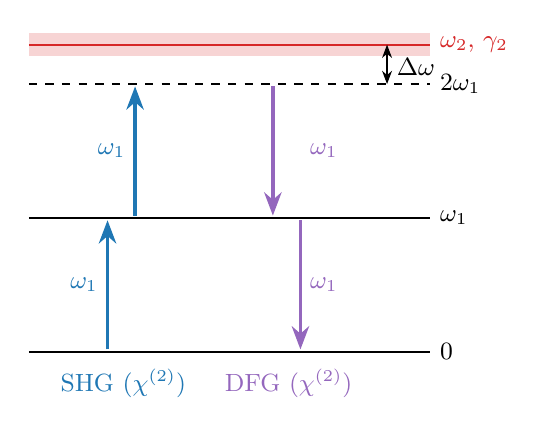
\begin{tikzpicture}[x=1cm,y=1cm,>=Stealth, every node/.style={font=\small}]
        % levels
        \draw[thick] (0,0) -- (5.1,0);
        \node[right] at (5.1,0) {$0$};
        \draw[thick] (0,1.7) -- (5.1,1.7);
        \node[right] at (5.1,1.7) {$\omega_1$};
        \draw[dashed] (0,3.4) -- (5.1,3.4);
        \node[right] at (5.1,3.4) {$2\omega_1$};
        % SH mode with linewidth band
        \fill[sh!20] (0,3.75) rectangle (5.1,4.05);
        \draw[thick,sh] (0,3.9) -- (5.1,3.9);
        \node[right,sh] at (5.1,3.9) {$\omega_2$, $\gtwo$};
        % detuning
        \draw[<->] (4.55,3.4) -- (4.55,3.9);
        \node[right] at (4.55,3.62) {$\Dom$};
        % SHG up arrows
        \draw[->,very thick,up] (1.0,0.03) -- (1.0,1.67);
        \draw[->,very thick,up] (1.35,1.73) -- (1.35,3.37);
        \node[left,up] at (1.0,0.85) {$\omega_1$};
        \node[left,up] at (1.35,2.55) {$\omega_1$};
        % DFG down arrows
        \draw[->,very thick,dn] (3.1,3.37) -- (3.1,1.73);
        \draw[->,very thick,dn] (3.45,1.67) -- (3.45,0.03);
        \node[right,dn] at (3.45,2.55) {$\omega_1$};
        \node[right,dn] at (3.45,0.85) {$\omega_1$};
        \node[up] at (1.2,-0.4) {SHG $(\chitwo)$};
        \node[dn] at (3.3,-0.4) {DFG $(\chitwo)$};
      \end{tikzpicture}
    \end{column}
    \begin{column}{0.54\linewidth}
      \footnotesize
      The SH is \textbf{virtual}: detuned by $\Dom = 2\omega_1-\omega_2$ from a dark,
      high-$Q_2$ mode, it never radiates; it only back-acts on the pump.
      A second-order process through the SH Green's function,
      \vspace{-4pt}
      \[
        \chicasc \;=\; \chitwo\cdot{\color{good}G(2\omega_1)}\cdot\chitwo,
        \qquad
        {\color{good}G} \;\propto\; \frac{\mathbf f_2(\mathbf r)\,\mathbf f_2^{*}(\mathbf r')}{\Dom + i\gtwo/2},
      \]
      \vspace{-10pt}

      which, reduced to the single dark mode, gives
      \vspace{-4pt}
      \[
        \boxed{\;\chicasc(\Dom) = -\,\frac{\omega_1\,|\chitwo|^2\,\eta_{\rm geom}}
                                          {6\,n_2^2\,\bigl(\Dom + i\gtwo/2\bigr)}\;}
      \]
      \vspace{-8pt}
      \begin{itemize}\setlength\itemsep{1pt}
        \item $\mathrm{Re}$: a Kerr response, $\propto 1/\Dom$,
              \textbf{sign-tunable} (focusing $\leftrightarrow$ defocusing);
        \item $\mathrm{Im}$: a two-photon-like loss, Lorentzian at $\Dom=0$:
              a \emph{detunable} saturable absorber;
        \item $\eta_{\rm geom}$: the $\chitwo$-weighted overlap of the two modes,
              the principal design parameter.
      \end{itemize}
    \end{column}
  \end{columns}
\end{frame}

% ---------------------------------------------------------------
\begin{frame}{Figure of merit: enhancement over the native Kerr}
  \vspace{-2pt}
  \[
    R \equiv \frac{|\chicasc|}{|\chinat|}, \qquad
    \chicasc\Bigr|_{\Dom=2\gtwo} \simeq \frac{Q_2}{24\,n_2^2}\,|\chitwo|^2\,\eta_{\rm geom}
  \]
  \vspace{-10pt}
  \begin{columns}[T]
    \begin{column}{0.55\linewidth}
      \centering
      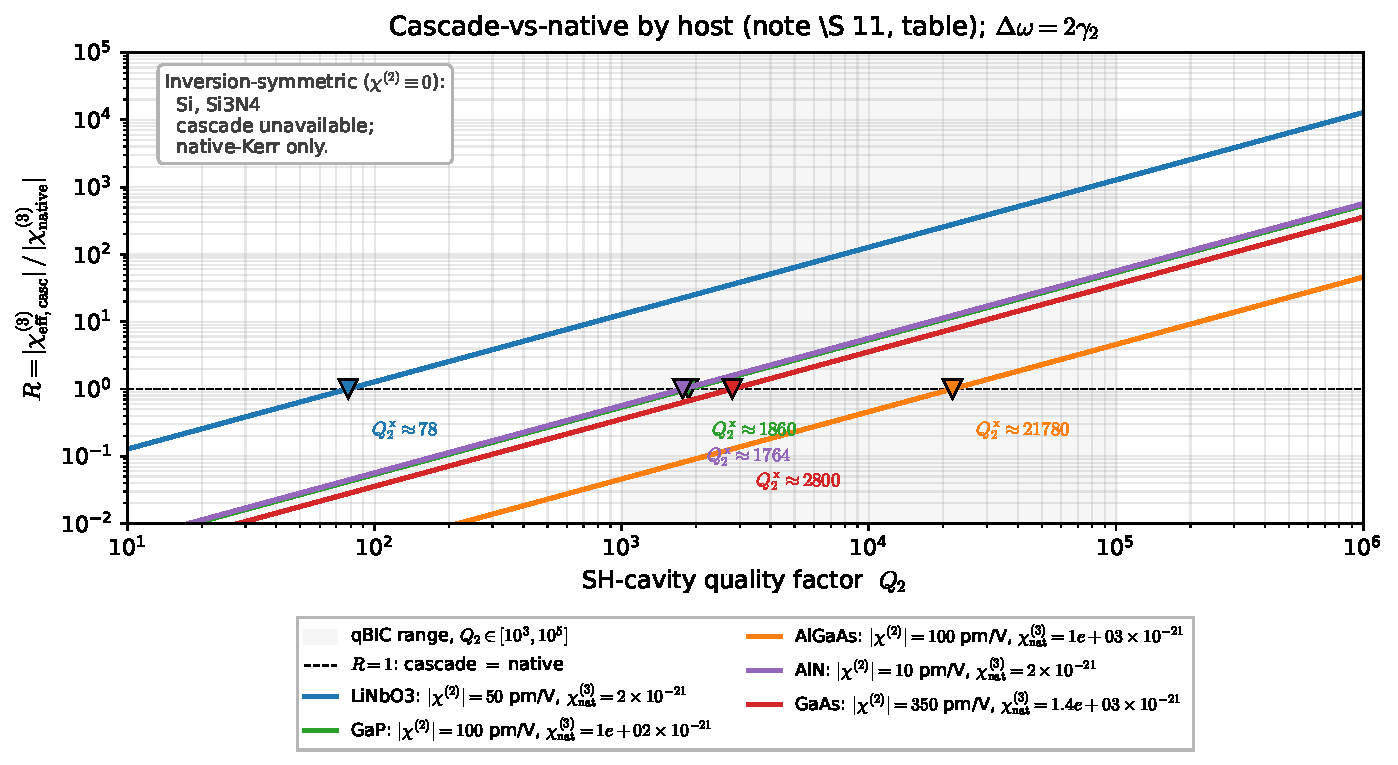
\includegraphics[width=0.92\linewidth]{cascaded_vs_native}
\end{column}
    \begin{column}{0.45\linewidth}
      \small
      \begin{table}
      \footnotesize
      \begin{tabular}{@{}lcc@{}}
        \toprule
        Host & $R$ @ $Q_2{=}4000$ & crossover $Q_2$ \\
        \midrule
        \textbf{LiNbO$_3$} & $\bm{\approx 12}$ & $\sim\!3\times10^2$ \\
        GaP     & 0.5  & $\sim\!7\times10^3$ \\
        AlN     & 0.6  & $\sim\!7\times10^3$ \\
        AlGaAs  & 0.05 & $\sim\!9\times10^4$ \\
        \bottomrule
      \end{tabular}
      \end{table}
      \vspace{2pt}
      LiNbO$_3$ is the favourable host \emph{because} its native Kerr is weak
      (crossover $Q_2\sim300$); the framework extends to the materials in our
      program (outlook slide).

      {\footnotesize \emph{Uncertainty:} absolute $R$ carries an $O(1)$ prefactor
      uncertainty; scalings and ratios are robust.}
    \end{column}
  \end{columns}
\end{frame}

% ===============================================================
\section{Platform and theory}

% ---------------------------------------------------------------
\begin{frame}{Platform: engineer the \emph{second-harmonic} resonance}
  \begin{columns}[T]
    \begin{column}{0.46\linewidth}
      \centering
      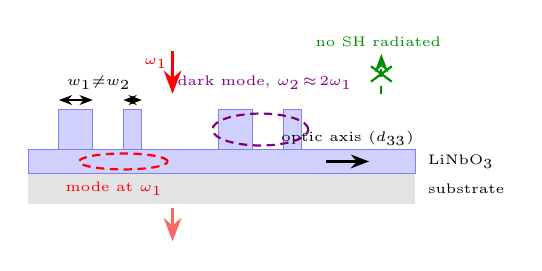
\begin{tikzpicture}[x=0.78cm,y=0.78cm,>=Stealth,every node/.style={font=\tiny}]
        % substrate and LN film (labels at the right margin, outside the structure)
        \fill[gray!22] (0,0) rectangle (6.3,0.5);
        \fill[blue!18] (0,0.5) rectangle (6.3,0.9);
        \node[right] at (6.35,0.7) {LiNbO$_3$};
        \node[right] at (6.35,0.25) {substrate};
        % two unit cells of asymmetric pillar pairs (w1 != w2)
        \foreach \xo in {0.5, 3.1} {
          \fill[blue!18] (\xo,0.9) rectangle ({\xo+0.55},1.55);
          \fill[blue!18] ({\xo+1.05},0.9) rectangle ({\xo+1.35},1.55);
          \draw[blue!50] (\xo,0.9) rectangle ({\xo+0.55},1.55);
          \draw[blue!50] ({\xo+1.05},0.9) rectangle ({\xo+1.35},1.55);
        }
        \draw[blue!50] (0,0.5) rectangle (6.3,0.9);
        % asymmetry annotation above cell 1
        \draw[<->] (0.5,1.7) -- (1.05,1.7);
        \draw[<->] (1.55,1.7) -- (1.85,1.7);
        \node at (1.15,1.98) {$w_1{\neq}w_2$};
        % optic axis in the slab, right side
        \draw[->,thick] (4.85,0.7) -- (5.55,0.7);
        \node at (5.2,1.08) {optic axis ($d_{33}$)};
        % FM mode (red) in slab, SH mode (violet) in pillars of cell 2
        \draw[red,thick,densely dashed] (1.55,0.7) ellipse (0.72 and 0.13);
        \node[red] at (1.4,0.26) {mode at $\omega_1$};
        \draw[violet,thick,densely dashed] (3.78,1.22) ellipse (0.78 and 0.26);
        \node[violet] at (3.85,1.98) {dark mode, $\omega_2\!\approx\!2\omega_1$};
        % pump in / transmitted, between the cells
        \draw[->,very thick,red] (2.35,2.5) -- (2.35,1.8);
        \node[red] at (2.08,2.3) {$\omega_1$};
        \draw[->,very thick,red!60] (2.35,-0.05) -- (2.35,-0.6);
        % no SH radiated, right of cell 2
        \draw[->,thick,green!55!black,dashed] (5.75,1.8) -- (5.75,2.45);
        \draw[green!55!black,thick] (5.58,2.0) -- (5.92,2.25);
        \draw[green!55!black,thick] (5.58,2.25) -- (5.92,2.0);
        \node[green!55!black] at (5.7,2.65) {no SH radiated};
      \end{tikzpicture}
    \end{column}
    \begin{column}{0.54\linewidth}
      \footnotesize
      \textbf{An inversion of our usual design philosophy}: the resonance that does
      the work sits at the \textbf{SH}, not at the pump.
      \begin{itemize}\setlength\itemsep{1pt}
        \item symmetry-protected qBIC at $\omega_2\approx2\omega_1$: high $Q_2$,
              \emph{dark} (no SH radiates); meta-atom asymmetry = the $Q_2$ knob;
        \item LiNbO$_3$ thin film, $x$-cut: $d_{33}$ with $E\parallel$ optic axis;
              fabrication constraints already in the designs;
        \item pump non-resonant (\textbf{singly resonant, 1R}) or sharing a qBIC
              (\textbf{doubly resonant, 2R}).
      \end{itemize}
    \end{column}
  \end{columns}
  \vspace{-2pt}
  \centering
  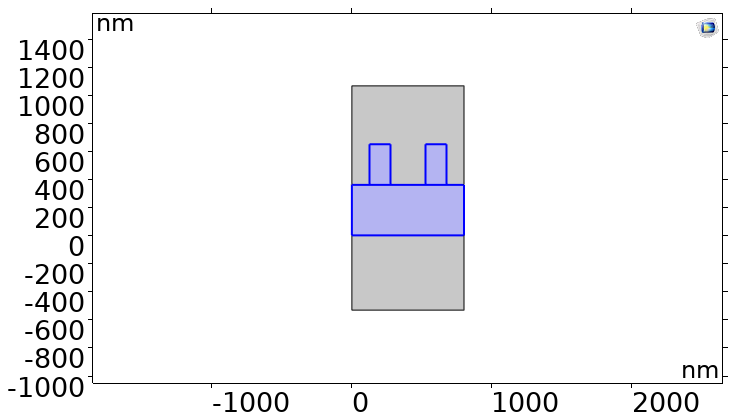
\includegraphics[height=2.35cm]{ln_unitcell_comsol}\hspace{14pt}%
  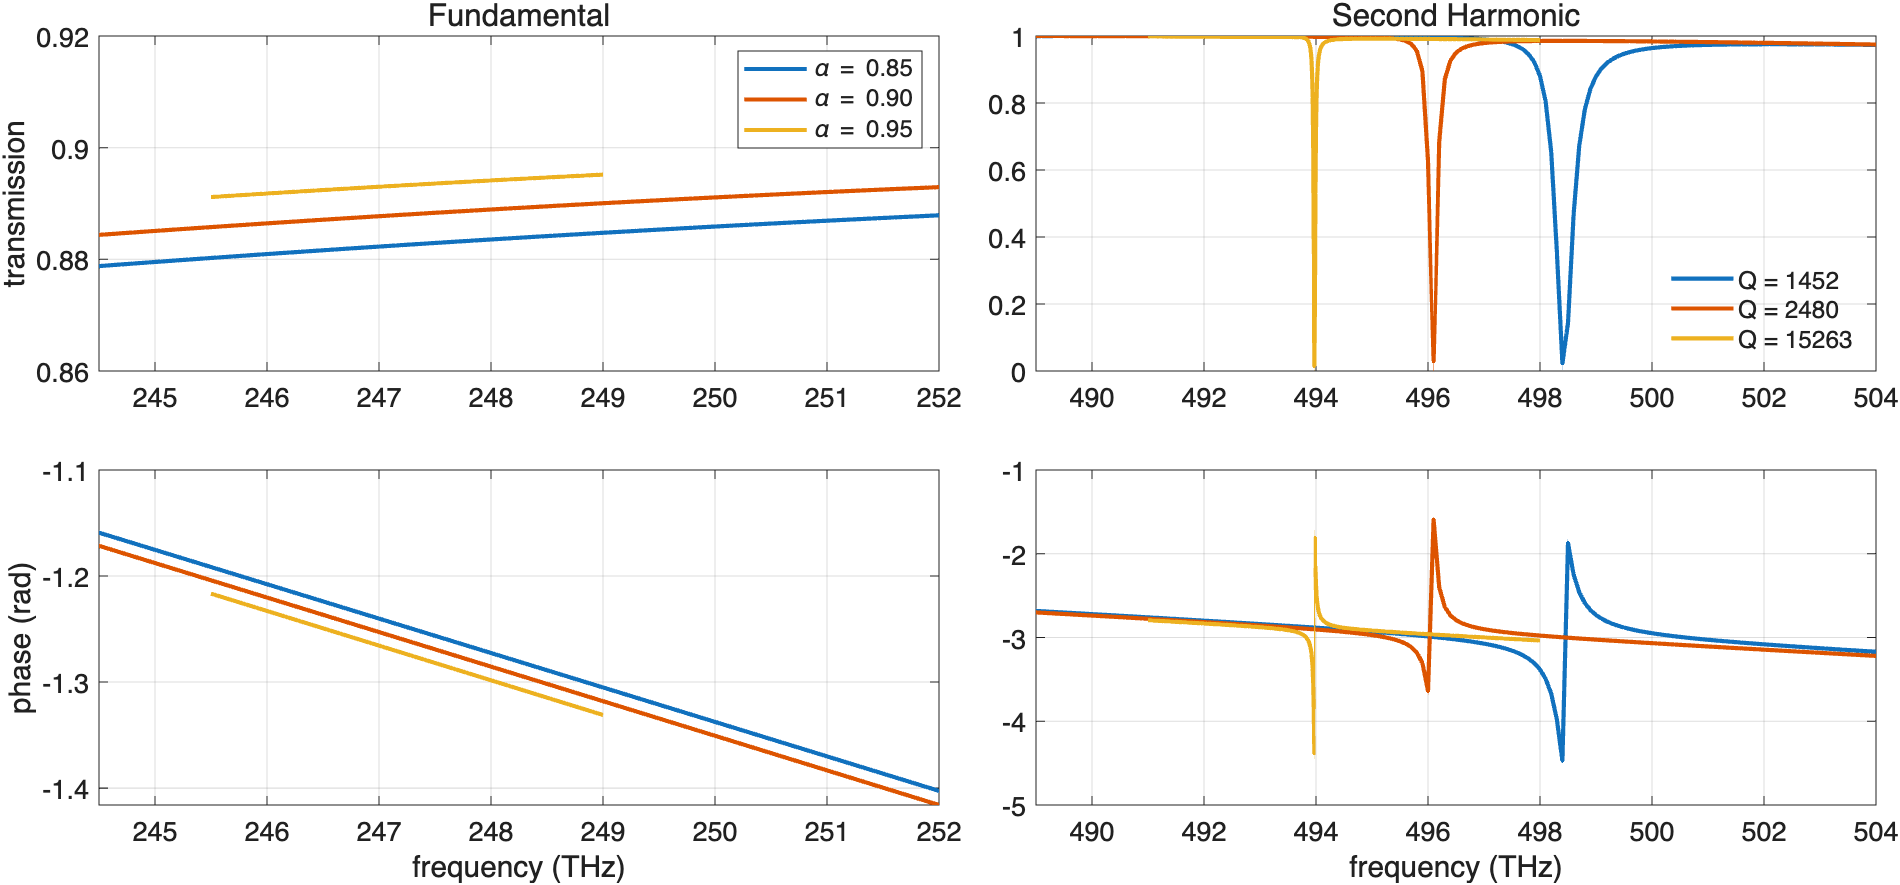
\includegraphics[height=2.35cm]{sh_qbic_asymmetry}
  \\[-1pt]
  {\footnotesize Unit cell (COMSOL); FM band featureless, SH qBIC $Q$ tuned
   $10^3$--$10^4$ by the asymmetry.}
\end{frame}

% ---------------------------------------------------------------
\begin{frame}{Theory in two lines (coupled-mode equations)}
  \vspace{-4pt}
  \[
    \frac{da_2}{dt} = \Bigl(i\Dom - \tfrac{\gtwo}{2}\Bigr) a_2 + i\beta\,a_1^2,
    \qquad
    \frac{da_1}{dt} = -\tfrac{\gone}{2}\,a_1 + i\beta^{*}a_1^{*}a_2
      + i\alpha_3 |a_1|^2 a_1 + \sqrt{\gamma_1^{\rm rad}}\,s_+
  \]
  {\small The \emph{same} $\beta$ in SHG and DFG terms $\Rightarrow$ Manley--Rowe.
  Adiabatic elimination of $a_2$ (valid for $|\Dom|\gtrsim2\gtwo$):}
  \vspace{-4pt}
  \[
    \alpha_3^{\rm casc}(\Dom) = -\frac{|\beta|^2\,\Dom}{\Dom^2+(\gtwo/2)^2}
    \quad\text{(Kerr)}, \qquad
    \gamma_3^{\rm casc}(\Dom) = \frac{|\beta|^2\,\gtwo/2}{\Dom^2+(\gtwo/2)^2}
    \quad\text{(TPA-like)}
  \]
  \vspace{-8pt}
  \centering
  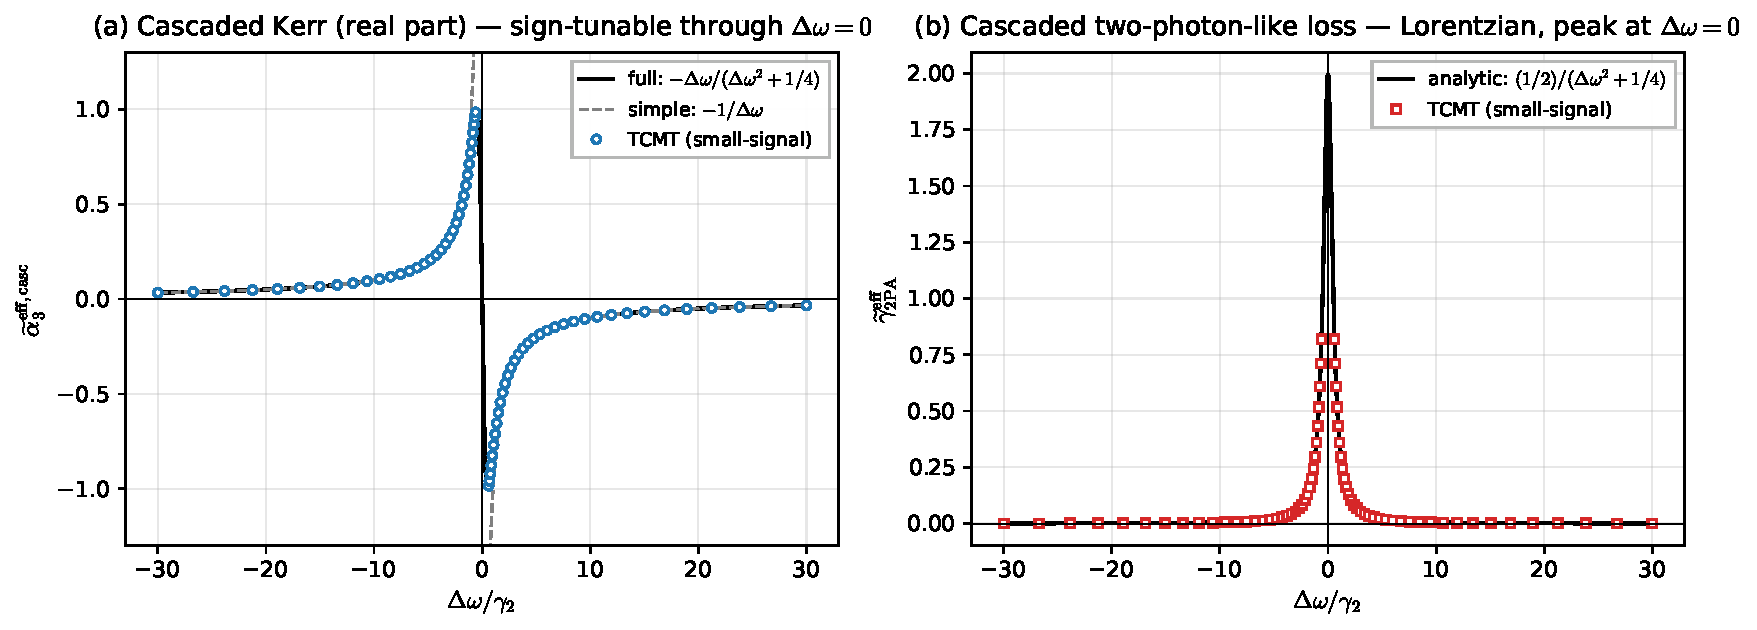
\includegraphics[width=0.66\linewidth]{validation}
  \\[-2pt]
  {\footnotesize Closed forms vs full nonlinear TCMT (circles/squares): exact agreement below saturation.}
\end{frame}

% ===============================================================
\section{Best case: the doubly-resonant metasurface}

% ---------------------------------------------------------------
\begin{frame}{Leverage on Kerr observables, and new capabilities}
  \small
  With the pump also resonant ($Q_1$), every Kerr observable inherits the cascade:
  \begin{columns}[T]
    \begin{column}{0.44\linewidth}
      \footnotesize
      \begin{table}
      \begin{tabular}{@{}lc@{}}
        \toprule
        Observable & gain vs native \\
        \midrule
        SPM / XPM phase & $1+R \approx 13$ \\
        Bistability threshold & $\tfrac{1}{1+R} \approx \tfrac{1}{13}$ \\
        Switching energy & $\tfrac{1}{1+R}$ \\
        \textbf{FWM efficiency} & $\bm{(1+R)^2 \approx 170}$ \\
        \bottomrule
      \end{tabular}
      \end{table}
      FWM is the most differentiating observable (TCMT-validated, backup).
      \vspace{3pt}
      \begin{table}
      \scriptsize
      \setlength{\tabcolsep}{3pt}
      \begin{tabular}{@{}ll@{}}
        \toprule
        Cascade-only & key property \\
        \midrule
        Saturable absorber & TPA peak $\propto Q_2$, detunable, ps \\
        Passive limiter & clamp at $|\beta a_1|=|\Dom|$ \\
        $\Dom$-readout sensor & slope $\propto Q_2^2$ ($Q_2^{3/2}$ shot-noise) \\
        \bottomrule
      \end{tabular}
      \end{table}
\end{column}
    \begin{column}{0.56\linewidth}
      \centering
      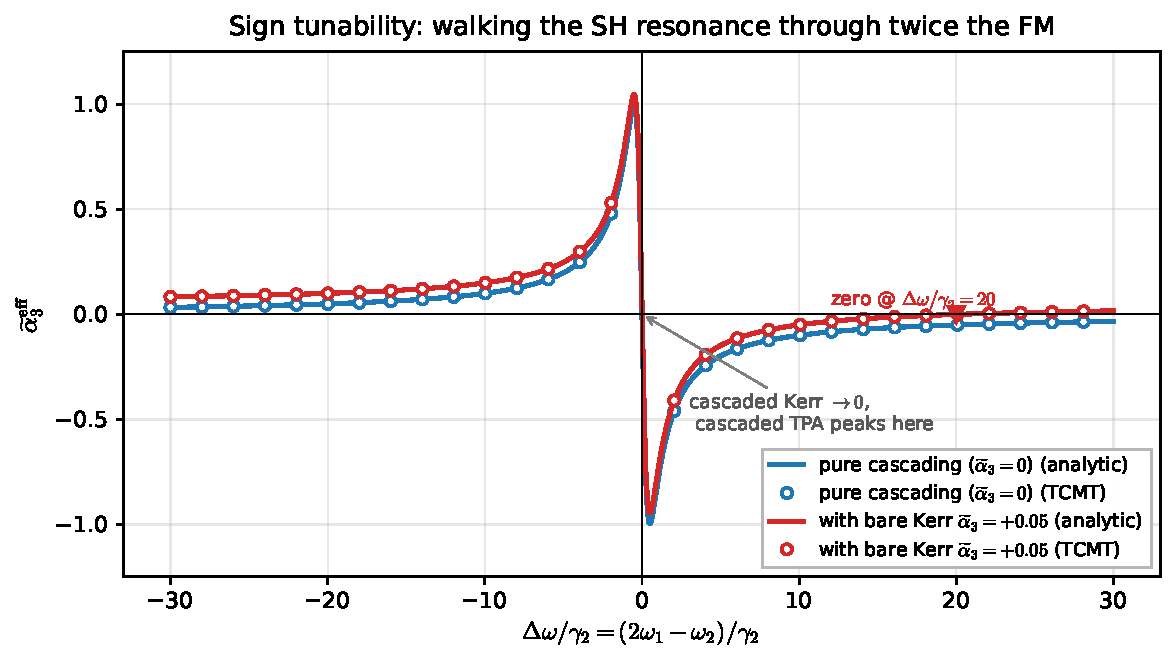
\includegraphics[width=0.9\linewidth]{sign_flip}
      \\[-2pt]
      {\footnotesize \textbf{Sign control}, unavailable in native Kerr:
       self-focusing $\leftrightarrow$ defocusing in one device
       (thermo-optic / Pockels tuning of $\omega_2$).}
\end{column}
  \end{columns}
\end{frame}

% ===============================================================
\section{Limitations and trade-offs}

% ---------------------------------------------------------------
\begin{frame}{Four intrinsic limitations}
  \begin{columns}[T]
    \begin{column}{0.5\linewidth}
      \small
      \begin{enumerate}\setlength\itemsep{5pt}
        \item \textbf{Cascaded TPA.} Loss/Kerr $= \gtwo/(2|\Dom|)$: $1/4$ at the
              conservative $\Dom=2\gtwo$; a loss channel absent in native LiNbO$_3$.
        \item \textbf{Sum rule.} $|\chicasc|_{\rm peak}\times\Delta f$ is fixed:
              $Q_2$ only reshapes the Lorentzian. Bandwidth $\approx100$\,GHz at
              $Q_2=4000$; ultrafast operation is excluded.
        \item \textbf{Saturation ceiling.} Parametric instability at
              $|\beta a_1|=|\Dom|$: usable pump window $\approx 1$ decade at $Q_2=4000$,
              shrinking as $1/Q_2^2$.
        \item \textbf{Speed} $\sim 1/\gtwo \sim$ ps: fine for CW/GHz, closed to fs
              applications.
      \end{enumerate}
    \end{column}
    \begin{column}{0.5\linewidth}
      \centering
      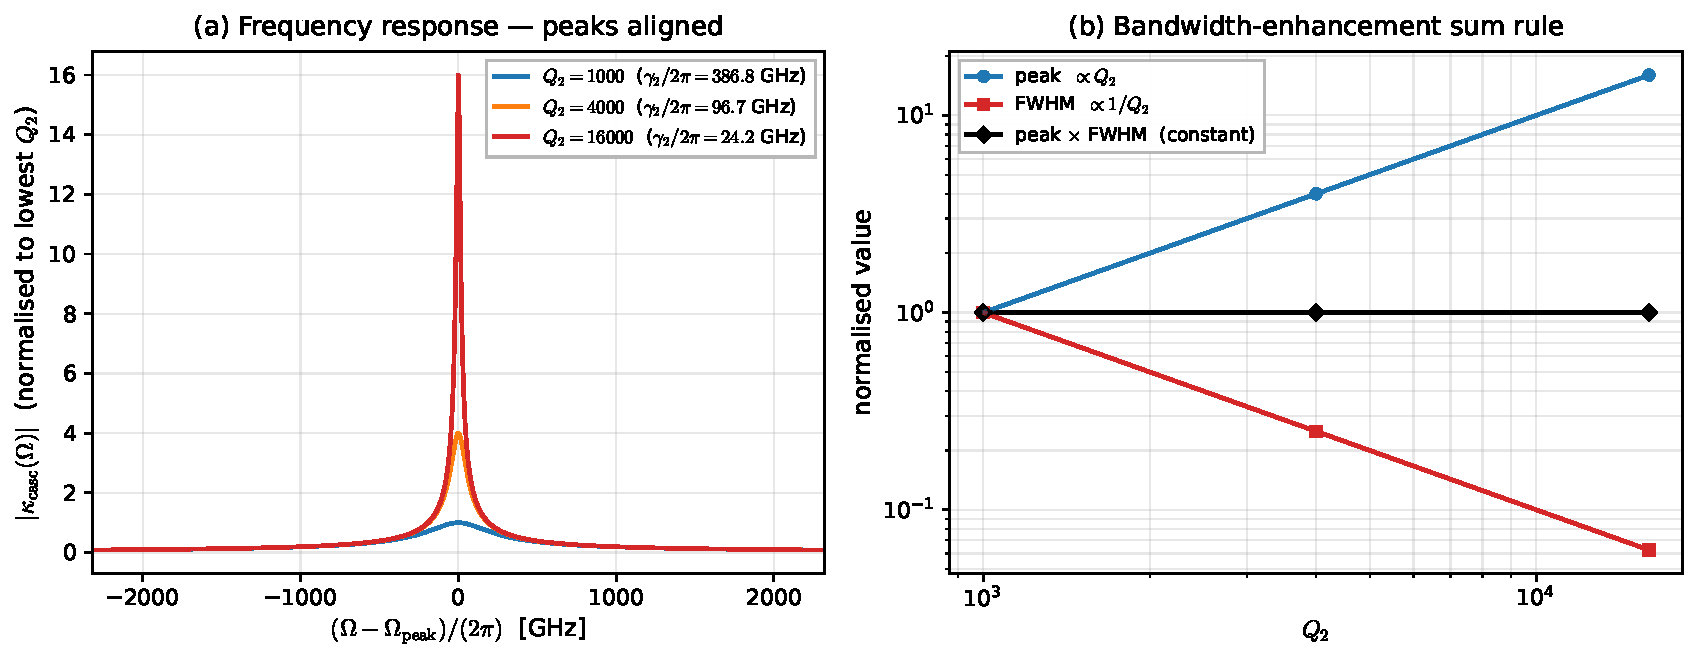
\includegraphics[width=\linewidth]{sum_rule}
      \\[2pt]
      {\footnotesize Peak $\propto Q_2$, FWHM $\propto 1/Q_2$, product constant:
       you cannot beat the sum rule by pushing $Q_2$.}
    \end{column}
  \end{columns}
\end{frame}

% ---------------------------------------------------------------
\begin{frame}{Fabrication constraints: the case for starting singly-resonant}
  \small
  \textbf{The doubly-resonant device needs:} two co-localised high-$Q$ modes,
  $\omega_2$ aligned to $2\omega_1$ against material dispersion, a tensor-correct
  overlap, \emph{and} array uniformity:
  \[
    Q_2^{\rm array} \;\text{collapses once}\;\; \sigma_\omega/\omega \gtrsim 1/Q_2
    \qquad (\text{sub-nm uniformity of the symmetry-breaking feature}).
  \]
  \begin{columns}[T]
    \begin{column}{0.55\linewidth}
      \begin{block}{Design study (full-wave, LiNbO$_3$)}
        \begin{itemize}\setlength\itemsep{2pt}
          \item \textbf{Doubly resonant:} $Q_2\approx5000$ achievable with
                $\sim$10\,\% overlap; mode alignment is the main difficulty.
          \item \textbf{Singly resonant:} $Q_2\approx8000$ with $\sim$20\,\% overlap;
                substantially easier, tunable by asymmetry alone.
        \end{itemize}
      \end{block}
    \end{column}
    \begin{column}{0.45\linewidth}
      \small
      \vspace{6pt}
      $\Rightarrow$ \textbf{strategy:} demonstrate and calibrate the cascade on the
      \emph{singly-resonant} platform first; develop the doubly-resonant design in
      parallel for the eventual Kerr device.
    \end{column}
  \end{columns}
\end{frame}

% ===============================================================
\section{The singly-resonant implementation}

% ---------------------------------------------------------------
\begin{frame}{What survives with only the SH resonance}
  \small
  \begin{table}
  \begin{tabular}{@{}lcc@{}}
    \toprule
     & doubly resonant (2R) & SH-only (1R) \\
    \midrule
    $\chicasc$, same boxed form & \yes & \yes \\
    Sign flip in $\Dom$ (the fingerprint) & \yes & \yes \\
    Detunable TPA / saturable loss & \yes & \yes \\
    $R>1$ (beat the native Kerr) & \yes & \yes\ \ (if overlap is good) \\
    Pump-cavity leverage $\sim Q_1^2$ on $\varphi_{\rm NL}$ & \yes & \no\ \ (single pass: $\mu$rad) \\
    Bistability, parametric ceiling, CW device & \yes & \no \\
    \bottomrule
  \end{tabular}
  \end{table}
  \vspace{4pt}
  \begin{alertblock}{Role of the 1R experiment}
    Not a device, but a \textbf{materials-level demonstration and calibration} of
    $\chicasc$: measure the sign flip, extract the magnitude, validate the model that
    the 2R device design rests on.
  \end{alertblock}
\end{frame}

% ---------------------------------------------------------------
\begin{frame}{Five fabricable singly-resonant designs}
  \begin{columns}[T]
    \begin{column}{0.42\linewidth}
      \small
      \begin{table}
      \footnotesize
      \setlength{\tabcolsep}{3.5pt}
      \begin{tabular}{@{}lccccc@{}}
        \toprule
        & $\lambda_1$ & $Q_2$ & overlap & $R$ & $>$1? \\
        \midrule
        S1 & 997\,nm  & 3442 & 0.12 & 0.49 & \no \\
        S2 & 975\,nm  & 3486 & 0.11 & 0.39 & \no \\
        S3 & 1058\,nm & 4641 & 0.19 & 1.76 & \yes \\
        S4 & 1064\,nm & 5633 & 0.21 & \textbf{2.49} & \yes \\
        \textcolor{d6}{\textbf{D6}} & \textbf{1757\,nm} & \textbf{924} & \textbf{0.43} & \textbf{1.81} & \yes \\
        \bottomrule
      \end{tabular}
      \end{table}
      \vspace{2pt}
      {\footnotesize
      S1--S4: pure-LiNbO$_3$ pillars (height asymmetry); \textcolor{d6}{\textbf{D6}}:
      TiO$_2$/LiNbO$_3$ hybrid (etch-angle asymmetry). Operating point $\Dom=+2\gtwo$;
      $R \propto Q_2 \times \mathrm{overlap}^2$.}
    \end{column}
    \begin{column}{0.58\linewidth}
      \centering
      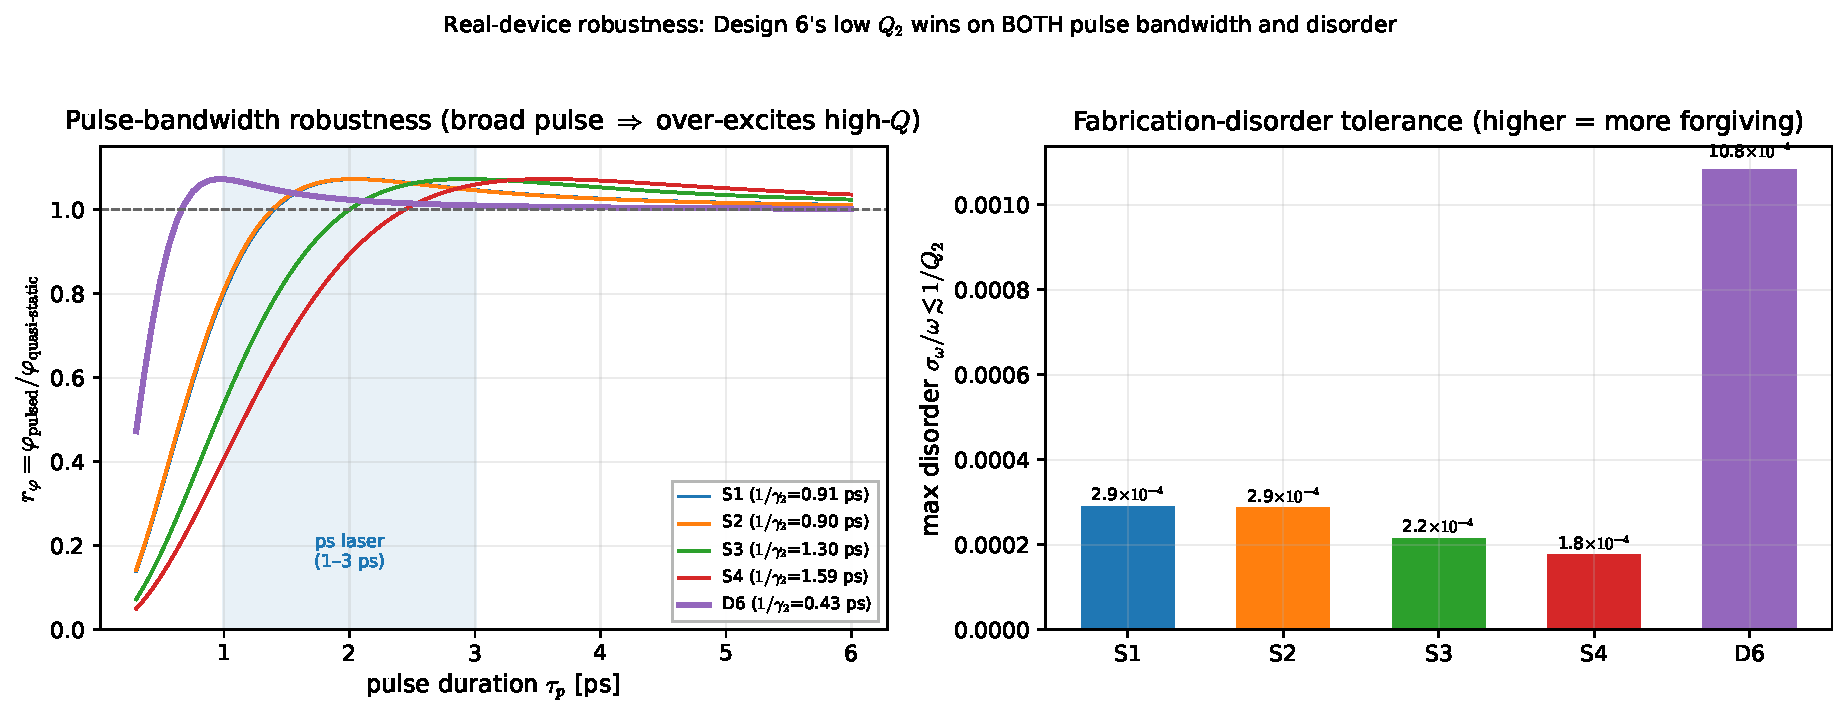
\includegraphics[width=0.93\linewidth]{combined_real_device}
      \vspace{1pt}
      \footnotesize
      A 1--3\,ps pulse is spectrally broad: high-$Q$ designs generate up to
      \textbf{22\,\%} of the SH at the \emph{wrong} sign of $\Dom$ (cancellation), so
      S4's Kerr phase drops to $0.4\times$ at 1\,ps.
      \textcolor{d6}{\textbf{D6}} is unaffected ($r_\varphi\!\approx\!1$) and
      tolerates $5\times$ more fabrication disorder.
    \end{column}
  \end{columns}
  \vspace{2pt}
  \begin{center}
    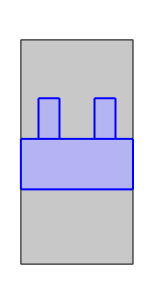
\includegraphics[height=1.3cm]{ln_cell_cut}\,{\scriptsize S1--S4}\hspace{12pt}%
    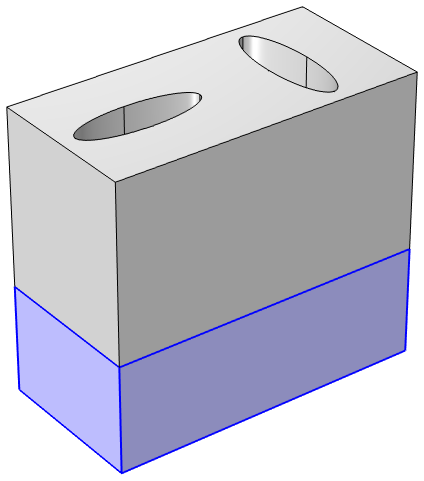
\includegraphics[height=1.3cm]{design6_cell_cut}\,{\scriptsize\textcolor{d6}{\textbf{D6}}}\hspace{14pt}%
    \raisebox{0.42cm}{\parbox{6.8cm}{\small
      \textbf{Best in the ideal limit: S4 ($R=2.49$).\\
      Best for a real device: \textcolor{d6}{D6} ($R\approx1.8$, robust).}}}
  \end{center}
\end{frame}

% ---------------------------------------------------------------
\begin{frame}{Proposed experiment: a resonant analogue of the 1992 Z-scan}
  \begin{columns}[T]
    \begin{column}{0.47\linewidth}
      \footnotesize
      \textbf{Closed-aperture Z-scan vs pump detuning}: the DeSalvo (1992) KTP
      measurement with the phase-match angle replaced by a \emph{resonance} detuning.
      \begin{itemize}\setlength\itemsep{2pt}
        \item tune the pump by a few nm $\Rightarrow$ the generated $2\omega_1$ sweeps
              across the SH mode, $\Dom: -\!\to\!+$;
        \item valley--peak $\to$ peak--valley reversal at $\Dom=0$: the cascade is
              \emph{odd} in $\Dom$, native Kerr a constant background;
              $R>1$ $\Rightarrow$ the \emph{total} $n_2$ reverses sign;
        \item SHG efficiency on the same sample pins the absolute $\chithree$ scale.
      \end{itemize}
      \begin{block}{Vehicle: \textcolor{d6}{Design 6} at $\lambda_1\approx1.76\,\mu$m}
        ps laser reaches it; SH lifetime $0.43$\,ps $\Rightarrow$ quasi-static at
        $\tau_p=1$--3\,ps; sign flip stays sharp.
      \end{block}
\end{column}
    \begin{column}{0.53\linewidth}
      \centering
      % --- Z-scan layout ---
      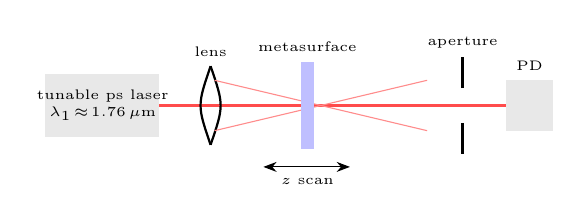
\begin{tikzpicture}[x=1cm,y=1cm,>=Stealth,every node/.style={font=\tiny}]
        \draw[red!70,line width=1.1pt] (1.3,0) -- (6.0,0);
        \fill[gray!18] (-0.15,-0.4) rectangle (1.3,0.4);
        \node[align=center] at (0.58,0) {tunable ps laser\\ $\lambda_1\!\approx\!1.76\,\mu$m};
        % lens
        \draw[thick] (1.95,-0.5) .. controls (2.12,0) .. (1.95,0.5);
        \draw[thick] (1.95,-0.5) .. controls (1.78,0) .. (1.95,0.5);
        \node at (1.95,0.68) {lens};
        % focus cone
        \draw[red!45] (2.0,0.32) -- (3.35,0) -- (4.7,0.32);
        \draw[red!45] (2.0,-0.32) -- (3.35,0) -- (4.7,-0.32);
        % sample on z stage
        \fill[blue!25] (3.1,-0.55) rectangle (3.26,0.55);
        \node at (3.18,0.75) {metasurface};
        \draw[<->] (2.62,-0.78) -- (3.72,-0.78);
        \node at (3.18,-0.97) {$z$ scan};
        % aperture
        \draw[thick] (5.15,0.22) -- (5.15,0.62);
        \draw[thick] (5.15,-0.22) -- (5.15,-0.62);
        \node at (5.15,0.8) {aperture};
        % detector
        \fill[gray!18] (5.7,-0.32) rectangle (6.3,0.32);
        \node at (6.0,0.5) {PD};
      \end{tikzpicture}
      \\[6pt]
      % --- closed-aperture traces: the sign flip ---
      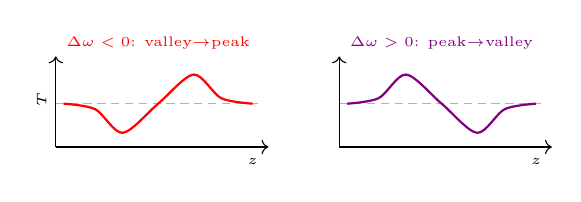
\begin{tikzpicture}[x=1cm,y=1cm,every node/.style={font=\tiny}]
        % left panel: focusing (valley -> peak)
        \draw[gray!60,densely dashed] (0,0.55) -- (2.6,0.55);
        \draw[->] (0,0) -- (2.7,0); \node at (2.5,-0.18) {$z$};
        \draw[->] (0,0) -- (0,1.15); \node[rotate=90] at (-0.18,0.6) {$T$};
        \draw[red,thick] plot[smooth] coordinates
          {(0.1,0.55) (0.5,0.48) (0.85,0.18) (1.3,0.55) (1.75,0.92) (2.1,0.62) (2.5,0.55)};
        \node[red] at (1.3,1.32) {$\Dom<0$: valley$\to$peak};
        % right panel: defocusing (peak -> valley)
        \begin{scope}[xshift=3.6cm]
          \draw[gray!60,densely dashed] (0,0.55) -- (2.6,0.55);
          \draw[->] (0,0) -- (2.7,0); \node at (2.5,-0.18) {$z$};
          \draw[->] (0,0) -- (0,1.15);
          \draw[violet,thick] plot[smooth] coordinates
            {(0.1,0.55) (0.5,0.62) (0.85,0.92) (1.3,0.55) (1.75,0.18) (2.1,0.48) (2.5,0.55)};
          \node[violet] at (1.3,1.32) {$\Dom>0$: peak$\to$valley};
        \end{scope}
      \end{tikzpicture}
      \\[-1pt]
      {\footnotesize The closed-aperture trace \emph{mirrors} as the pump crosses
       $\Dom=0$: the cascade's fingerprint. Predicted spectra: backup.}
    \end{column}
  \end{columns}
\end{frame}

% ===============================================================
\section{Outlook: the doubly-resonant device and new materials}

% ---------------------------------------------------------------
\begin{frame}{The doubly-resonant path: a first candidate}
  \begin{columns}[T]
    \begin{column}{0.5\linewidth}
      \centering
      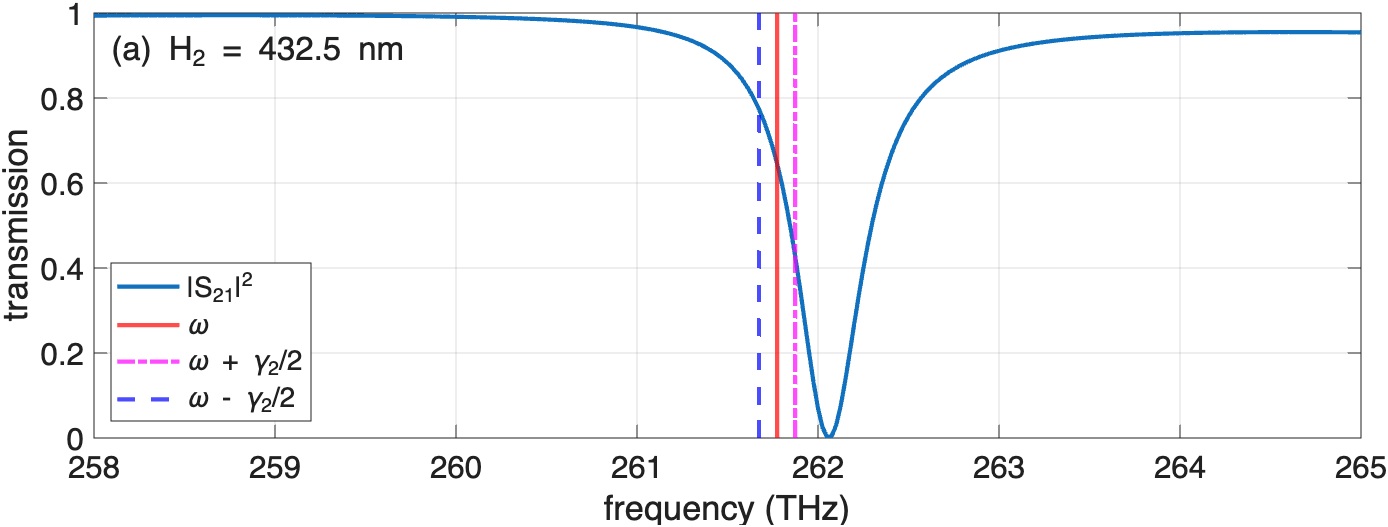
\includegraphics[width=\linewidth]{dr_candidate_fm}
      \\[-1pt]
      {\footnotesize Pump resonance at $\omega_1$; markers show the operating pump
       frequency and $\omega\pm\gtwo/2$ inside the line.}
    \end{column}
    \begin{column}{0.5\linewidth}
      \centering
      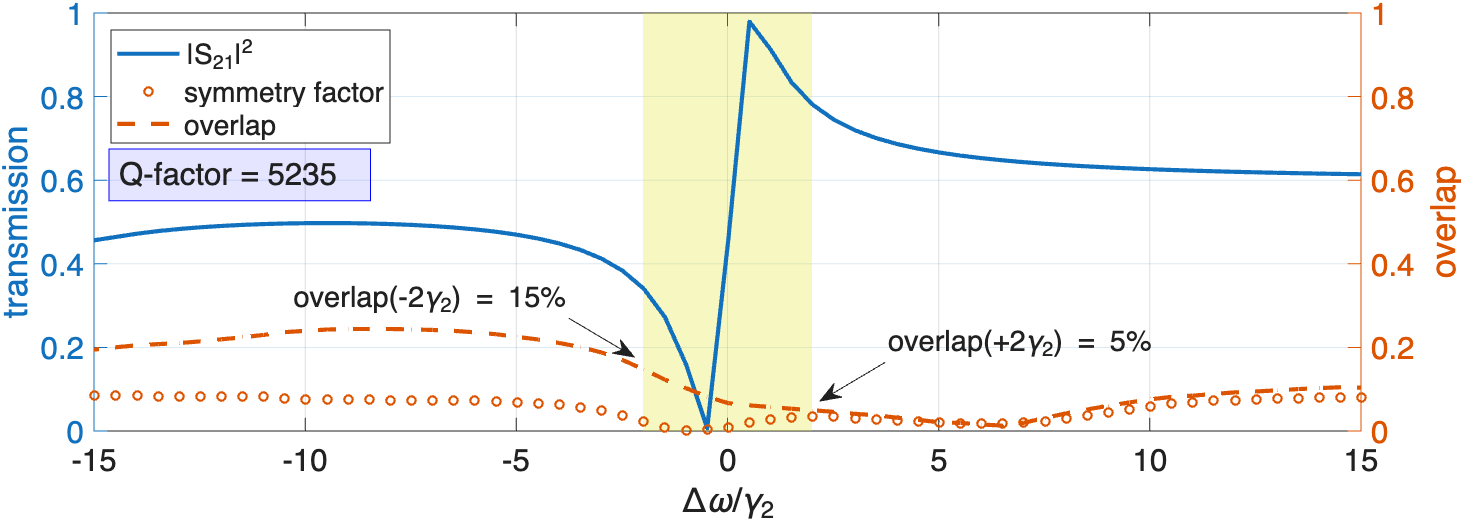
\includegraphics[width=\linewidth]{dr_candidate_sh}
      \\[-1pt]
      {\footnotesize SH qBIC: $Q_2=5235$, overlap 15\,\% at $\Dom=-2\gtwo$.}
    \end{column}
  \end{columns}
  \vspace{4pt}
  \begin{columns}[T]
    \begin{column}{0.85\linewidth}
      \small
      \begin{itemize}\setlength\itemsep{2pt}
        \item Full-wave design with \textbf{co-localised pump and SH modes}: the central
              difficulty of the 2R scheme is already solved at the design level.
        \item $Q_2\,\times\,\mathrm{overlap}^2$ comparable to the best singly-resonant
              samples, and the pump cavity restores the device-level leverage
              ($1{+}R$ phase, bistability, FWM).
        \item Observable-level analysis of this design is the next iteration; the 1R
              calibration fixes its absolute scale.
      \end{itemize}
    \end{column}
    \begin{column}{0.15\linewidth}
      \centering
      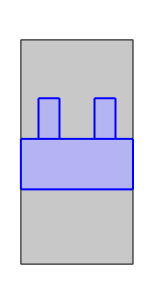
\includegraphics[height=2.0cm]{ln_cell_cut}
      \\[-1pt]
      {\tiny LN pillar-pair cell}
    \end{column}
  \end{columns}
\end{frame}

% ---------------------------------------------------------------
\begin{frame}{Beyond LiNbO$_3$: MURI material platforms}
  \small
  LiNbO$_3$ is the calibration baseline; the formalism is material-agnostic:
  $R \propto |\chitwo|^2\, Q_2\, \eta_{\rm geom}\, /\, \chi^{(3)}_{\rm native}$.
  \vspace{2pt}
  \begin{itemize}\setlength\itemsep{6pt}
    \item \textbf{III--V semiconductors (GaAs, GaP; MBE growth within the team).}
          Bulk $|\chitwo|$ up to $\sim$350\,pm/V; team-demonstrated interband
          coupled-QW $\chitwo$ up to 2750\,pm/V at $1.55\,\mu$m
          {\tiny\color{gray}(Ramesh \emph{et al.}, Optica, in press; arXiv:2602.23246)}.
          At telecom the band-edge native Kerr dominates ($R<1$);
          pumping \textbf{below half the gap} (mid-IR) suppresses the native Kerr by
          roughly an order of magnitude and removes intrinsic TPA
          ($2\hbar\omega < E_g$) $\Rightarrow$ $R>1$ at the same $Q_2$, with the SH
          still below the gap.
    \item \textbf{MQW intersubband metasurfaces} (our Nature 2014 platform):
          engineered $|\chitwo| \sim 5\times10^{4}$\,pm/V at $\lambda\approx8\,\mu$m;
          a natural \textbf{next step} for the cascade. The same quantum engineering
          must also \emph{suppress} the (equally giant) native intersubband
          $\chithree$; SH-band absorption sets $Q_2$.
    \item \textbf{Epitaxial BaTiO$_3$ on Si} (team growth): optical $d$ coefficients
          below LiNbO$_3$'s, but a giant Pockels response
          ($r_{\rm eff}$ up to $\sim$430\,pm/V): exactly the $\Dom$-tuning knob the
          cascade needs (sign flip, AM modulation), monolithic on Si.
          \hfill {\tiny\color{gray} Demkov group, JVST A \textbf{39}, 030804 (2021)}
  \end{itemize}
\end{frame}

% ===============================================================
\section{Honest summary}

% ---------------------------------------------------------------
\begin{frame}{Honest summary}
  \begin{columns}[T]
    \begin{column}{0.5\linewidth}
      \small
      \begin{block}{What is real today}
        \begin{itemize}\setlength\itemsep{1pt}
          \item $R \approx 1.8$--$2.5$ over native Kerr in fabricable single-resonance
                LiNbO$_3$ designs;
          \item a clean, unambiguous fingerprint: the \textbf{sign flip}, odd in $\Dom$;
          \item a robust vehicle (\textcolor{d6}{\textbf{D6}}): immune to pulse
                bandwidth and $5\times$ looser on disorder;
          \item validated theory: closed form = full TCMT.
        \end{itemize}
      \end{block}
    \end{column}
    \begin{column}{0.5\linewidth}
      \small
      \begin{block}{What is not (yet)}
        \begin{itemize}\setlength\itemsep{1pt}
          \item a CW Kerr \emph{device}: single-pass phase is $\mu$rad; this requires
                the doubly-resonant version ($1{+}R$ leverage, $R\sim12$);
          \item absolute $R$: order-of-magnitude until the SHG calibration pins the
                overlap normalisation;
          \item bandwidth beyond $\sim$100\,GHz: the sum rule forbids it.
        \end{itemize}
      \end{block}
    \end{column}
  \end{columns}
  \vspace{4pt}
  \begin{alertblock}{Next steps}
    \small
    \textbf{(1)} ps Z-scan sign-flip on Design 6 at $1.76\,\mu$m + SHG calibration
    (pins the absolute scale).
    \textbf{(2)} Advance the doubly-resonant candidate: the device-level payoff.
    \textbf{(3)} Realise the cascade on the MQW intersubband platform:
    quantum-engineered $\chitwo$ with the photonic $Q_2/\Dom$ lever.
  \end{alertblock}
\end{frame}

% ===============================================================
\appendix
\section*{Backup}

% ---------------------------------------------------------------
\begin{frame}{Backup: adiabatic elimination, explicitly}
  Setting $\dot a_2 \to 0$ for $|\Dom| \gtrsim 2\gtwo$: \quad
  $a_2 = -\beta\,a_1^2/(\Dom + i\gtwo/2)$, so that
  \[
    \frac{da_1}{dt} = -\tfrac{\gone}{2}a_1
      + i\Bigl[\alpha_3 - \frac{|\beta|^2\Dom}{\Dom^2+(\gtwo/2)^2}\Bigr]|a_1|^2a_1
      - \frac{|\beta|^2\gtwo/2}{\Dom^2+(\gtwo/2)^2}\,|a_1|^2a_1 + \sqrt{\gamma_1^{\rm rad}}s_+
  \]
  \[
    \beta = \frac{\varepsilon_0\omega_1}{4}\int \chi^{(2)}_{ijk}(\mathbf r)\,
            f^{*}_{2,i}f_{1,j}f_{1,k}\,d^3r,
    \qquad
    \alpha_3 = \frac{3\varepsilon_0\omega_1}{8}\int \chi^{(3)}_{ijkl}
            f^{*}_{1,i}f_{1,j}f_{1,k}f^{*}_{1,l}\,d^3r
  \]
  Modes are energy-normalised (Brillouin form
  $\widetilde\varepsilon = \partial(\omega\varepsilon_r)/\partial\omega$); $|a_n|^2$ =
  stored energy. Boyd degeneracy factors (SHG 1, DFG 2, SPM 3) are what make the same
  $\beta$ appear in both equations (Manley--Rowe).

  \vspace{4pt}
  \textbf{SH-only case:} the same elimination with the local (non-resonant) FM field gives
  \[
    \chi^{(3),{\rm 1R}}_{\rm casc}
      = -\,\frac{\varepsilon_0\,\omega_1\,|\widetilde M|^2}
                {6\,(\Dom+i\gtwo/2)\,V_{\rm cell}},
    \qquad \eta_{\rm geom}^{\rm 1R} = \bigl(|{\rm overlap}|/V\bigr)^2 .
  \]
\end{frame}

% ---------------------------------------------------------------
\begin{frame}{Backup: $\chicasc$ from the polarisation chain alone}
  \small
  No mode decomposition; three steps at the level of macroscopic polarisations
  (Boyd convention, $\mathcal E = \tfrac12[E e^{-i\omega t} + \mathrm{c.c.}]$):
  \begin{enumerate}\setlength\itemsep{2pt}
    \item \textbf{SHG drive:}\; $P^{(2)}(2\omega_1) = \varepsilon_0\,\chitwo\,E(\omega_1)^2$
          \hfill (single ordering, no degeneracy factor)
    \item \textbf{Propagation:}\;
          $E(2\omega_1;\mathbf r) = \mu_0(2\omega_1)^2 \displaystyle\int
          {\color{good}G(\mathbf r,\mathbf r';2\omega_1)}\;P^{(2)}(\mathbf r')\,d^3r'$,
          \hfill ($G$: Green's function of the wave operator at $2\omega_1$)
    \item \textbf{DFG return:}\; $P^{(3)}(\omega_1) = 2\,\varepsilon_0\,\chitwo\,
          E(2\omega_1)\,E^{*}(\omega_1)$ \hfill (two orderings, Boyd factor 2)
  \end{enumerate}
  Identifying with the SPM form $P^{(3)}(\omega_1) \equiv 3\varepsilon_0\,\chicasc\,|E|^2E$:
  \quad
  $\chicasc = \tfrac{2}{3}\,\mu_0(2\omega_1)^2\,
      \chitwo\!\cdot\!{\color{good}G(2\omega_1)}\!\cdot\!\chitwo$ \ (schematic).
  Two limits of ${\color{good}G}$ recover both regimes:
  \begin{itemize}\setlength\itemsep{2pt}
    \item \textbf{bulk SVEA} (phase-mismatch kernel):\;
          $\chi^{(3)}_{\rm casc,bulk} = -\dfrac{2\omega_1\,|\chitwo|^2 F}{3\,c\,n_2\,\Delta k}$,
          the PPLN regime;
    \item \textbf{single resonant mode} (QNM expansion):\;
          ${\color{good}G} \to \dfrac{c^2}{2\omega_2}\,
          \dfrac{\mathbf f_2(\mathbf r)\mathbf f_2^{*}(\mathbf r')}{\Dom+i\gtwo/2}$,
          giving the boxed metasurface result.
          \hfill {\tiny\color{gray} Sauvan \emph{et al.}, PRL 2013; Lalanne \emph{et al.}, LPR 2018}
  \end{itemize}
\end{frame}

% ---------------------------------------------------------------
\begin{frame}{Backup: two routes to $R\approx2$; Design 6 spectrum}
  \begin{columns}[T]
    \begin{column}{0.46\linewidth}
      \centering
      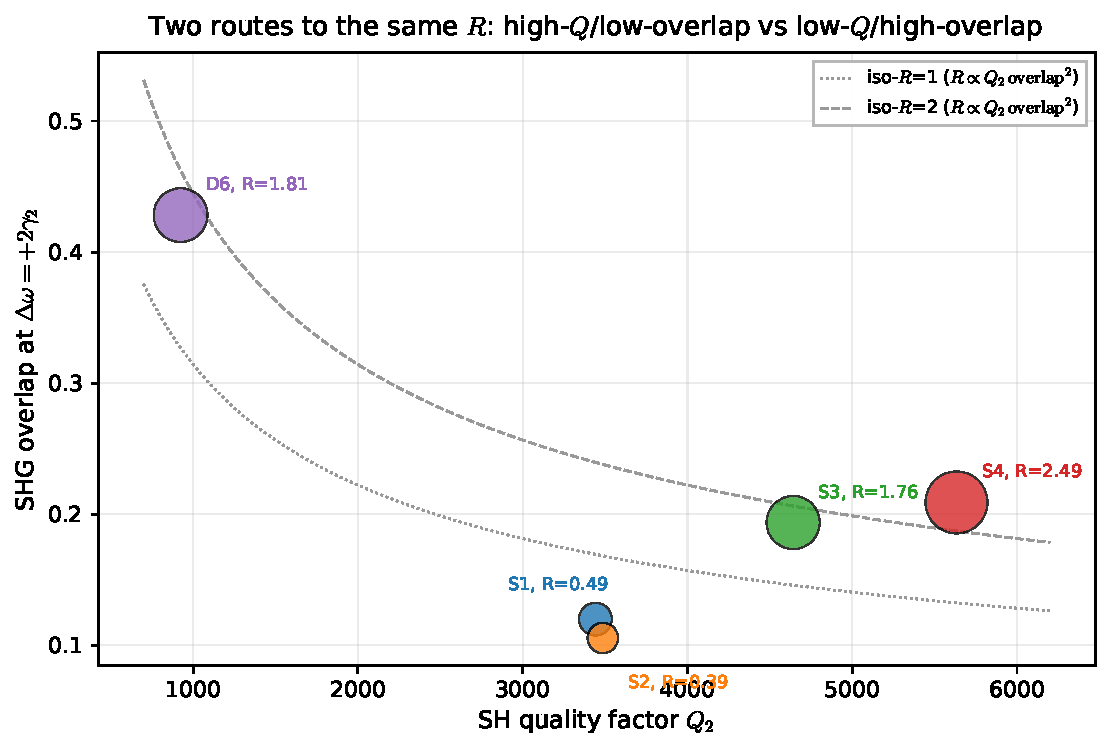
\includegraphics[width=\linewidth]{combined_tradeoff}
      \\[-1pt]
      {\footnotesize Iso-$R$ curves $R\propto Q_2\,\mathrm{overlap}^2$:
       S4 (high $Q$, low overlap) and D6 (low $Q$, high overlap) reach comparable $R$.}
    \end{column}
    \begin{column}{0.54\linewidth}
      \centering
      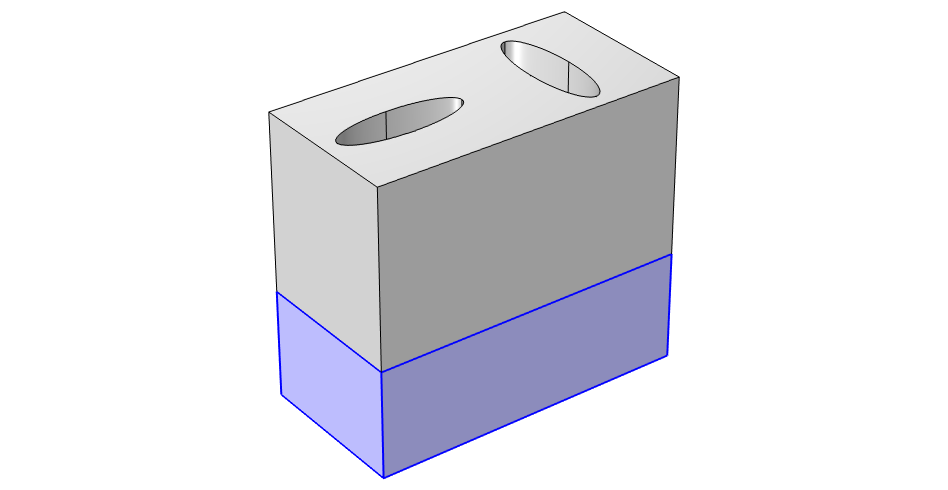
\includegraphics[width=0.42\linewidth]{design6_cell}
      \\[2pt]
      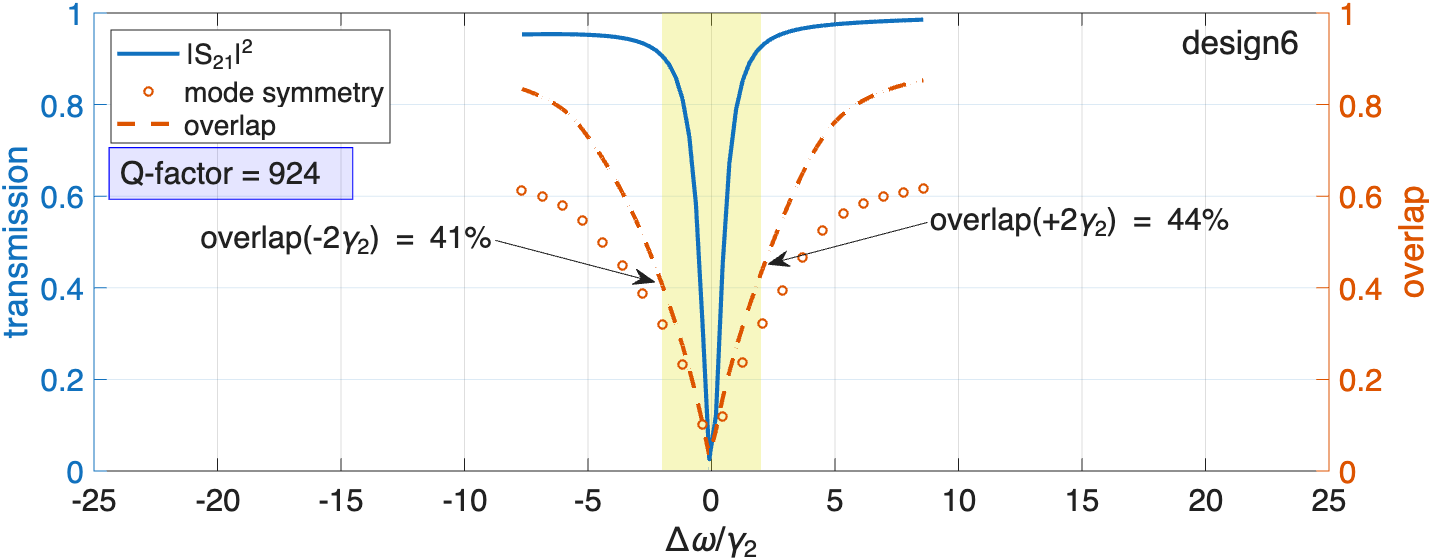
\includegraphics[width=\linewidth]{design6_spectrum}
      \\[-1pt]
      {\footnotesize \textcolor{d6}{\textbf{Design 6}}: $Q_2=924$, overlap $0.41/0.44$
       at $\mp2\gtwo$.}
    \end{column}
  \end{columns}
\end{frame}

% ---------------------------------------------------------------
\begin{frame}{Backup: FWM enhancement $(1+R)^2$, TCMT-validated}
  \centering
  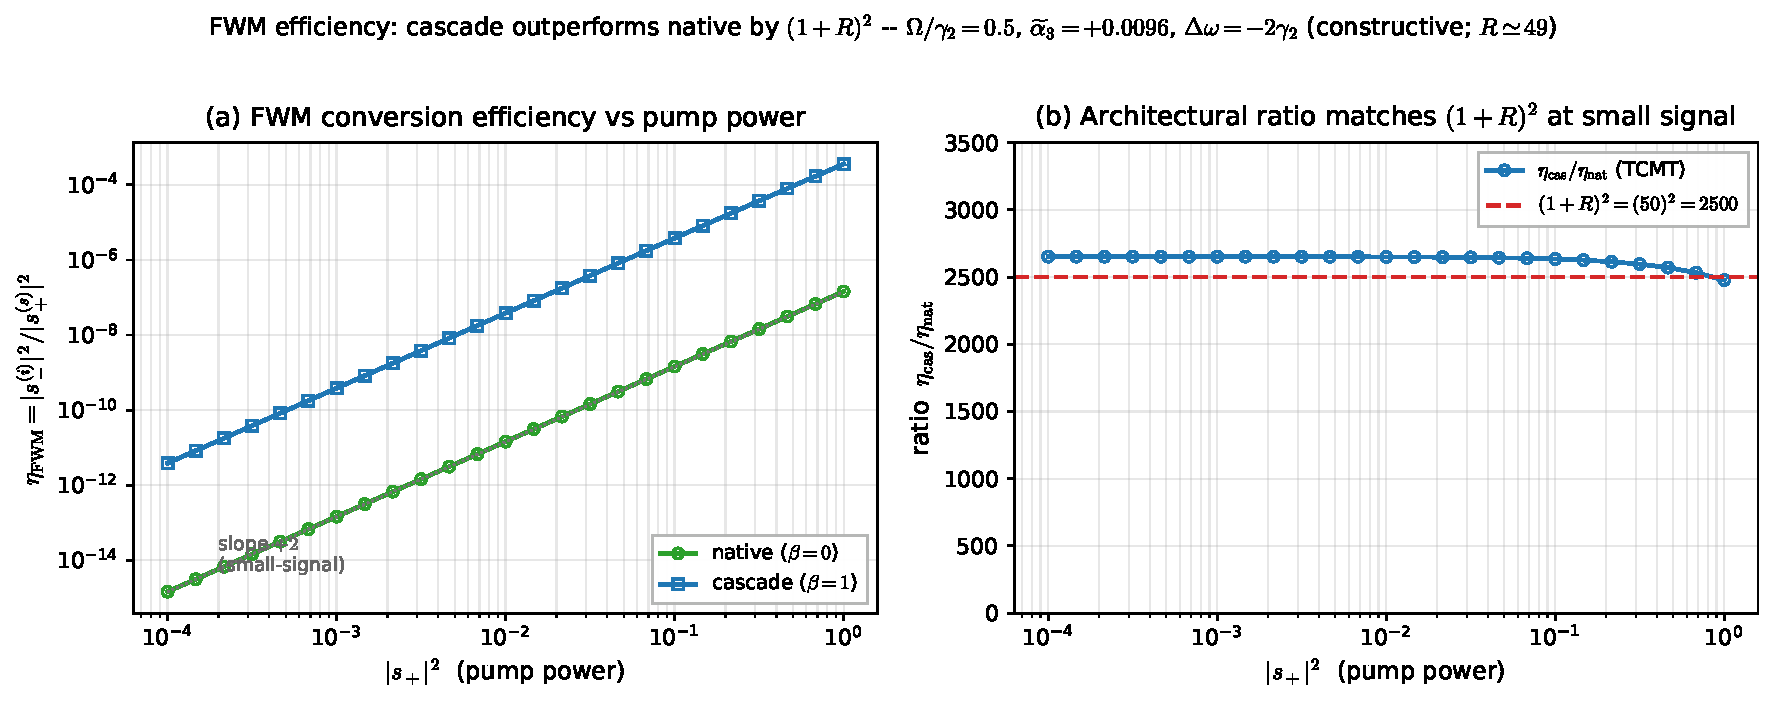
\includegraphics[width=0.86\linewidth]{fwm_efficiency}
  \\[2pt]
  {\footnotesize Pump + weak signal inside the fundamental linewidth; idler efficiency
   scales as $|\alpha_3^{\rm eff}|^2$, so the architectural ratio is $(1+R)^2 = 169$ at
   the LiNbO$_3$ design point. Validity: $\Omega < \min(\gone,\gtwo)$, small-signal
   cascade.}
\end{frame}

% ---------------------------------------------------------------
\begin{frame}{Backup: Design 6 predicted $\chithree$ spectra}
  \centering
  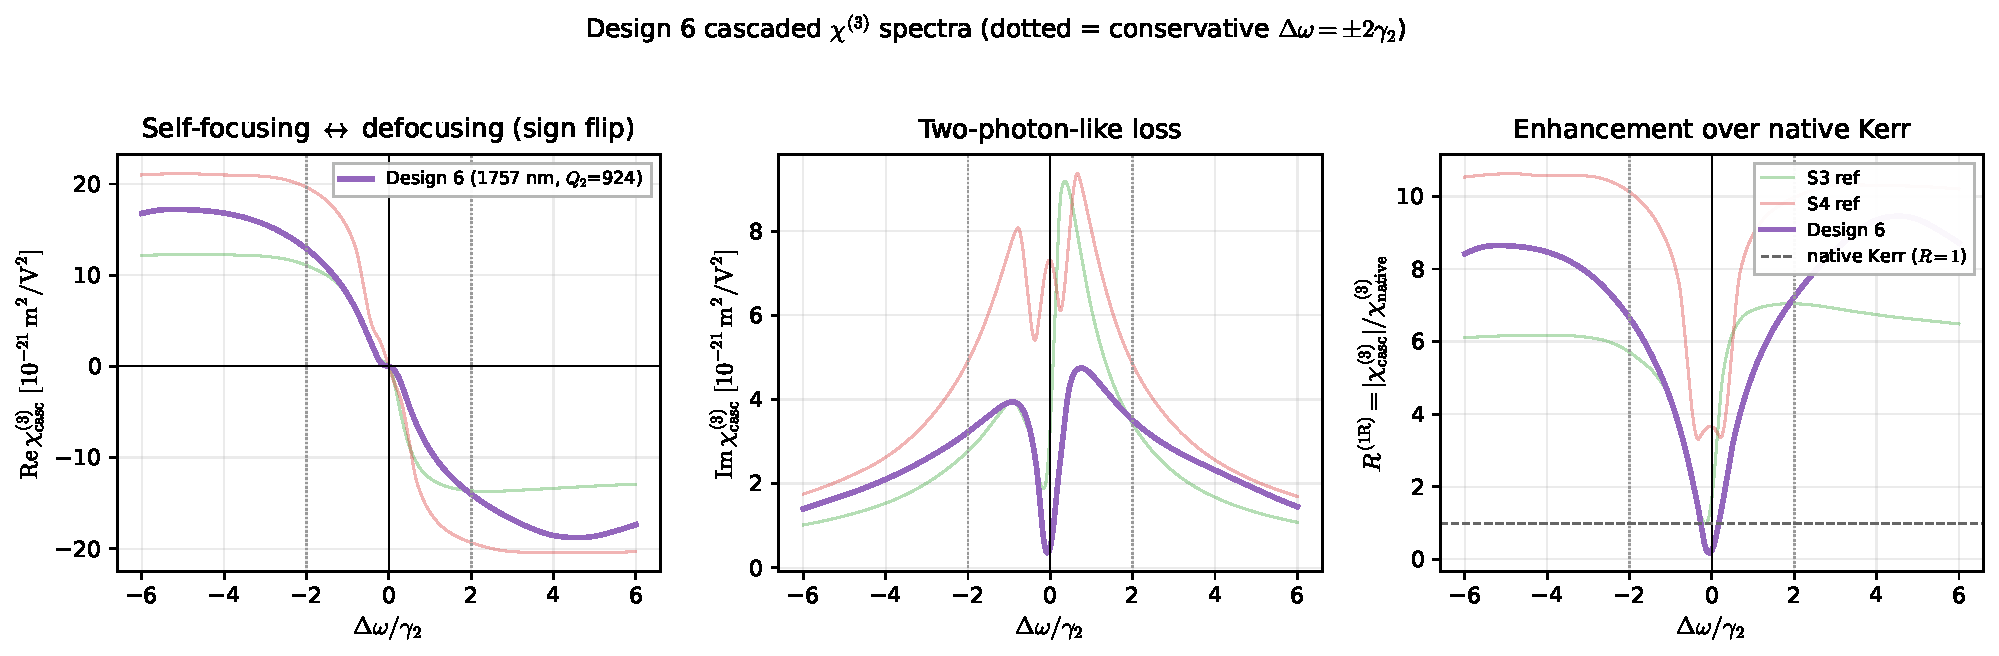
\includegraphics[width=0.98\linewidth]{design6_chi3_spectra}
  \\[2pt]
  {\footnotesize Sign-tunable Re\,$\chicasc$, Lorentzian-like Im\,$\chicasc$
   (two-photon-like loss), and $R$ up to $\sim$2.2--2.4 in the wings; dotted lines mark
   the conservative $\Dom=\pm2\gtwo$ operating points.}
\end{frame}

% ---------------------------------------------------------------
\begin{frame}{Backup: host-material survey}
  \small
  \begin{table}
  \begin{tabular}{@{}lccccc@{}}
    \toprule
    Host & $|\chitwo|$ [m/V] & $|\chinat|$ [m$^2$/V$^2$] & $n_2$ & $R$ @ $Q_2{=}4000$ & $Q_2^{\rm cross}$ \\
    \midrule
    LiNbO$_3$ & $5\times10^{-11}$   & $2\times10^{-21}$   & 2.26 & \textbf{12.8} & 313 \\
    GaP       & $1\times10^{-10}$   & $1\times10^{-19}$   & 3.05 & 0.54 & 7\,442 \\
    AlGaAs    & $1\times10^{-10}$   & $1\times10^{-18}$   & 3.30 & 0.05 & 87\,120 \\
    AlN       & $1\times10^{-11}$   & $2\times10^{-21}$   & 2.10 & 0.57 & 7\,060 \\
    GaAs      & $3.5\times10^{-10}$ & $1.4\times10^{-18}$ & 3.50 & 0.36 & 11\,200 \\
    Si, Si$_3$N$_4$ & 0 & --- & --- & --- (no cascade) & --- \\
    \bottomrule
  \end{tabular}
  \end{table}
  \vspace{4pt}
  Conservative operating point $\Dom = 2\gtwo$, $\eta_{\rm geom}=0.3$ assumed for all hosts.
  Semiconductors lose because their band-edge-enhanced \emph{native} Kerr is even larger
  than their $|\chitwo|^2$ advantage.
\end{frame}

% ---------------------------------------------------------------
\begin{frame}{Backup: dynamic range vs $Q_2$}
  \small
  Floor: readable phase $\varphi_{\rm NL}\gtrsim10$\,mrad. Ceiling: parametric
  instability $|\beta a_1| = |\Dom|$, $|a_1|^2_{\rm sat}\propto 1/Q_2^2$ at fixed
  $\Dom/\gtwo$.
  \begin{table}
  \begin{tabular}{@{}cccc@{}}
    \toprule
    $Q_2$ & $R$ & usable pump window & verdict \\
    \midrule
    1\,000  & $\approx3$   & $\sim$3 decades   & disorder-tolerant, modest gain \\
    4\,000  & $\approx12$  & $\sim$1 decade    & \textbf{design point} (already at the edge) \\
    10\,000 & $\approx30$  & $\sim$0.3 decade  & marginal \\
    $10^5$  & $\approx300$ & $\sim$0.03 decade & unusable \\
    \bottomrule
  \end{tabular}
  \end{table}
  \vspace{4pt}
  Want more leverage \emph{and} range? Increase $|\chitwo|$ or $\eta_{\rm geom}$,
  not $Q_2$.
\end{frame}

% ---------------------------------------------------------------
\begin{frame}{Backup: disorder / inhomogeneous broadening}
  \small
  qBIC arrays average over meta-atoms: the array linewidth collapses once
  $\sigma_\omega/\omega \gtrsim 1/Q_2$
  (equivalently $\sigma_\alpha/\alpha \lesssim 1\%$ for the headline 2R point).
  \begin{table}
  \begin{tabular}{@{}lccccc@{}}
    \toprule
     & S1 & S2 & S3 & S4 & \textcolor{d6}{\textbf{D6}} \\
    \midrule
    max $\sigma_\omega/\omega$ & $2.9\times10^{-4}$ & $2.9\times10^{-4}$
      & $2.2\times10^{-4}$ & $1.8\times10^{-4}$ & $\bm{1.1\times10^{-3}}$ \\
    \bottomrule
  \end{tabular}
  \end{table}
  \vspace{4pt}
  Mitigations for high-$Q$ routes: smaller pump spot / single-shot e-beam field,
  post-fabrication trimming, thermo-optic feedback, ensemble-averaged readout.
\end{frame}

% ---------------------------------------------------------------
\begin{frame}{Backup: Design 6 details}
  \begin{columns}[T]
    \begin{column}{0.5\linewidth}
      \centering
      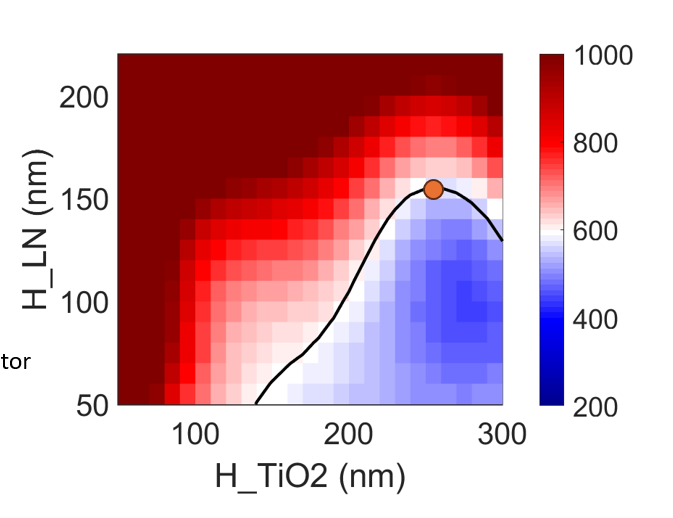
\includegraphics[width=0.72\linewidth]{design6_heatmap}
      \\[-2pt]
      {\footnotesize $Q_2$ over (H$_{\rm TiO_2}$, H$_{\rm LN}$); chosen point marked.}
      \\[4pt]
      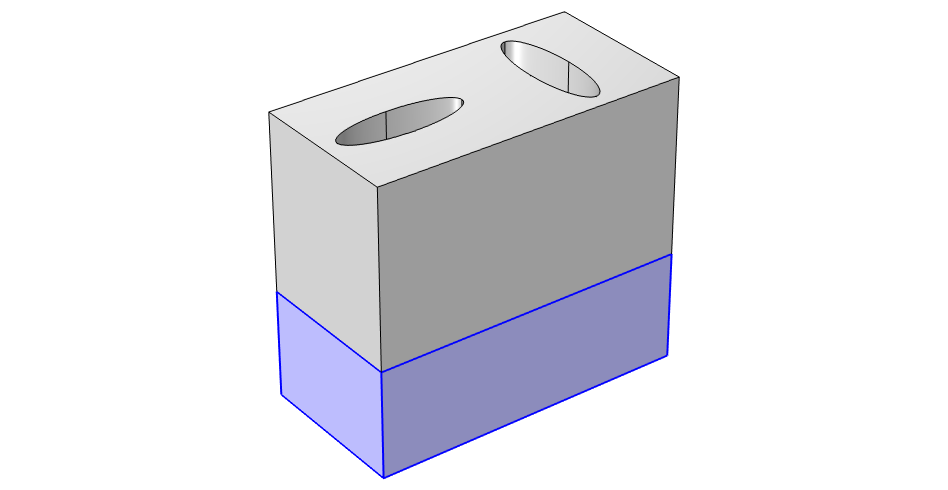
\includegraphics[width=0.55\linewidth]{design6_cell}
\end{column}
    \begin{column}{0.5\linewidth}
      \footnotesize
      \begin{itemize}\setlength\itemsep{2pt}
        \item TiO$_2$ pillars (two elliptical holes, etch angles $0^\circ/90^\circ$) on a
              \emph{solid} LiNbO$_3$ slab; only the LN is nonlinear.
        \item $H_{\rm LN}=150$\,nm, $H_{\rm TiO_2}=246$\,nm, axes $176\times58$\,nm,
              period 219\,nm ($2p\times p$ supercell).
        \item Optic axis in-plane ($\parallel x$): $E_x$ input, $d_{33}$ channel,
              $n_{1}=2.13$, $n_{2}=2.17$ ($n_e$); effective hybrid index within
              1\,\% of bare LN.
        \item Verified: Fano fit $Q=920$ vs quoted 924; volume $=2p^2H_{\rm LN}$ exact;
              overlap $0.41/0.44$ reproduced; FM transmission flat (0.98).
        \item Optimal detuning: $R$ peaks $\approx2.36$ at $\Dom\approx+4.5\gtwo$
              (overlap keeps rising in the wings).
      \end{itemize}
\end{column}
  \end{columns}
\end{frame}

% ---------------------------------------------------------------
\begin{frame}{Backup: sample spectra (S4) and pulsed response}
  \begin{columns}[T]
    \begin{column}{0.5\linewidth}
      \centering
      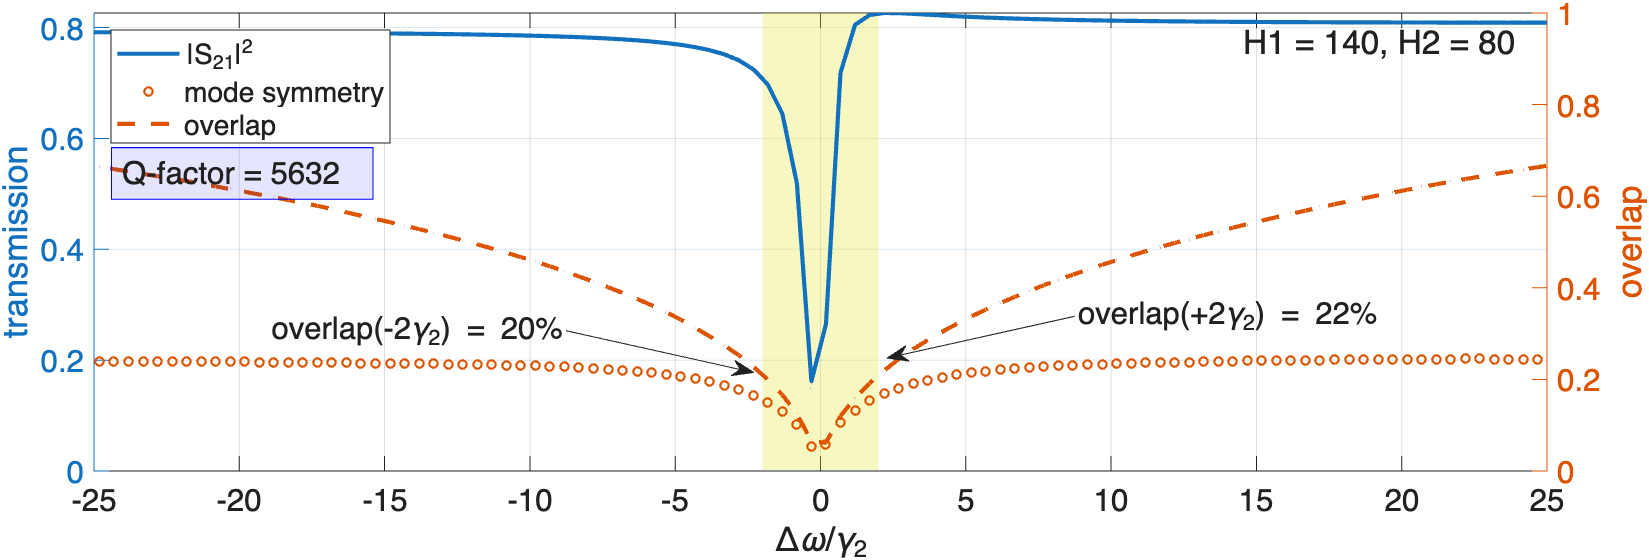
\includegraphics[width=\linewidth]{sample4_spectrum}
      \\[-2pt]
      {\footnotesize S4: $Q_2=5633$, overlap $0.20/0.22$ at $\mp2\gtwo$; the best
       design in the ideal limit.}
    \end{column}
    \begin{column}{0.5\linewidth}
      \centering
      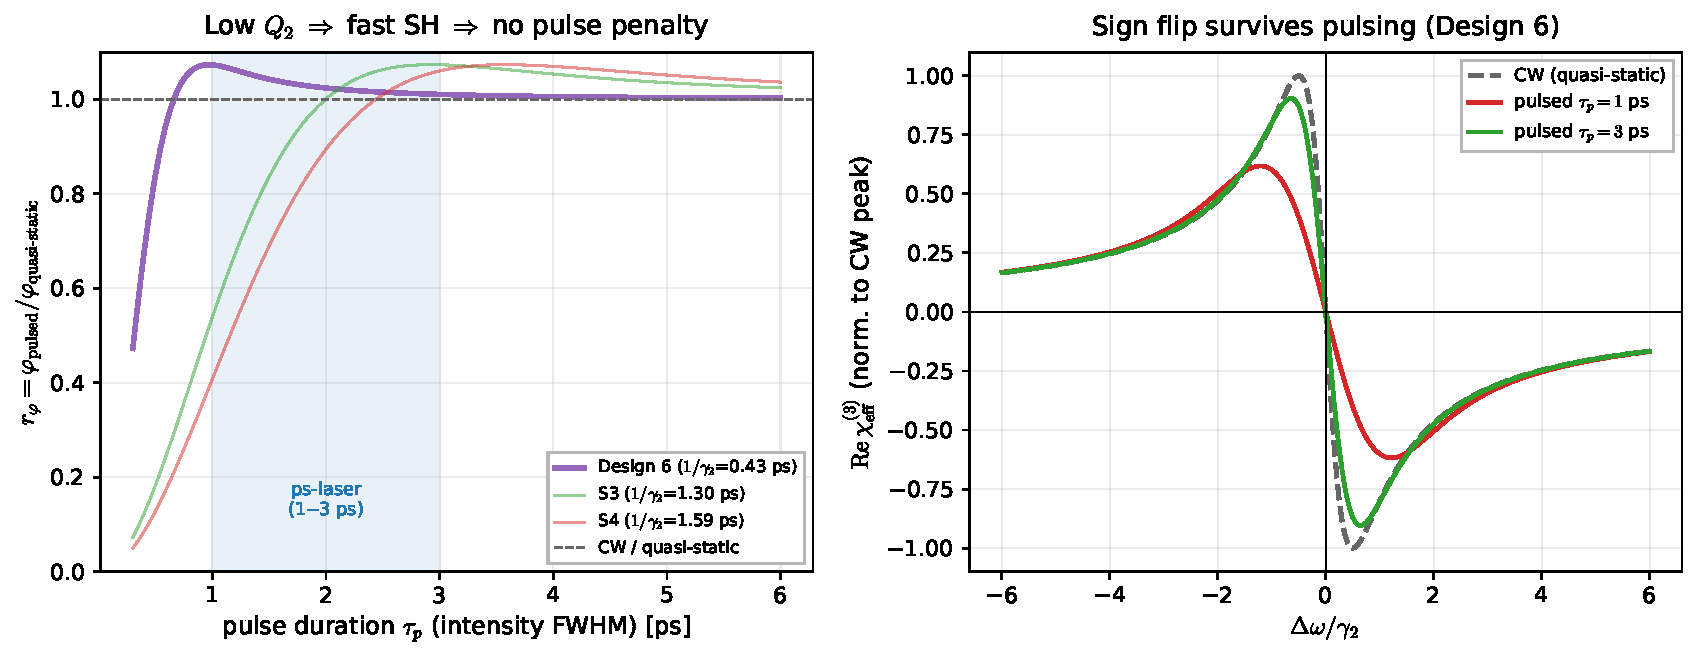
\includegraphics[width=\linewidth]{design6_pulsed}
      \\[-2pt]
      {\footnotesize D6 time-domain pulsed TCMT: quasi-static at 1--3\,ps
       ($r_\varphi = 1.07/1.02/1.01$), sign flip survives.}
    \end{column}
  \end{columns}
\end{frame}

% ---------------------------------------------------------------
\begin{frame}{Backup: doubly-resonant design progress}
  \begin{columns}[T]
    \begin{column}{0.5\linewidth}
      \centering
      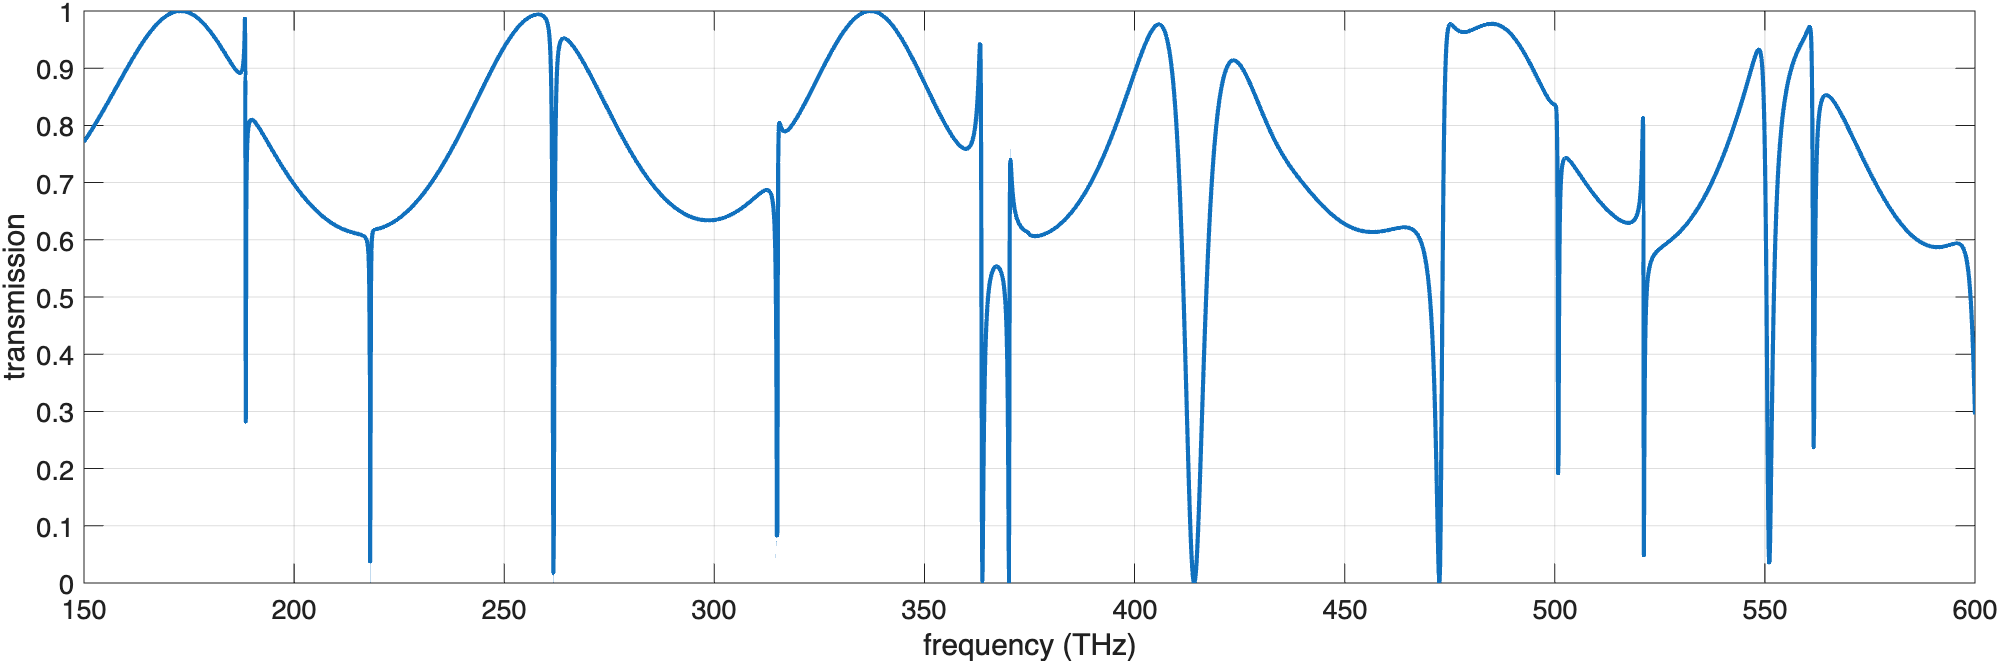
\includegraphics[width=\linewidth]{dr_design_a}
    \end{column}
    \begin{column}{0.5\linewidth}
      \centering
      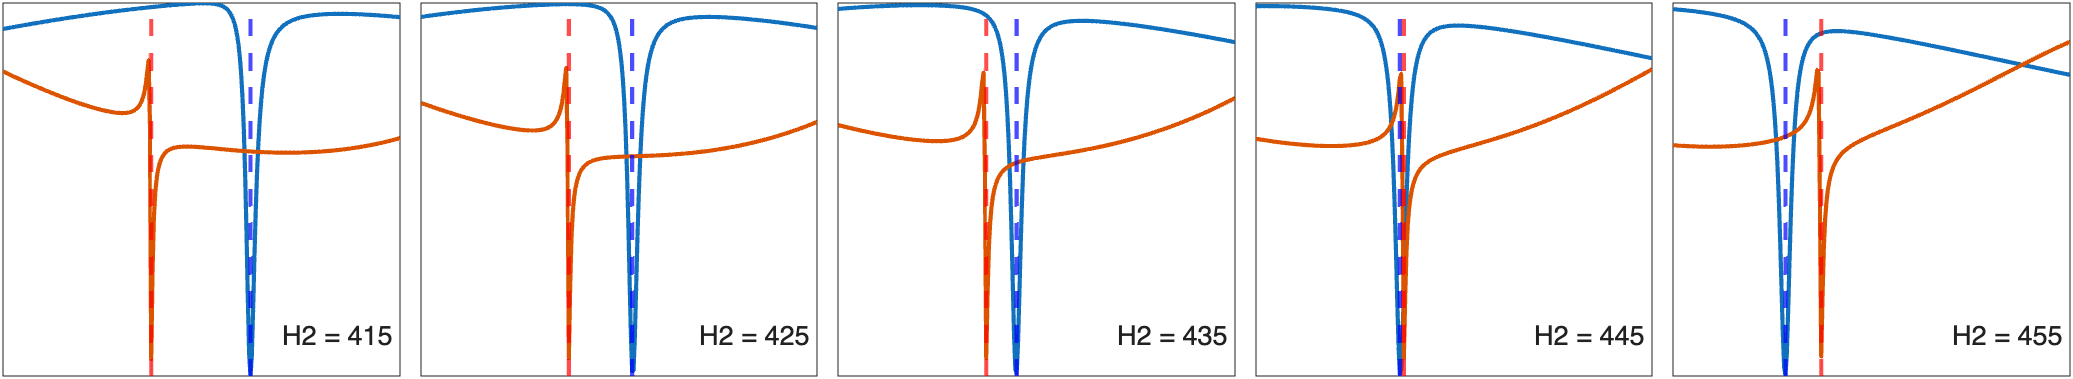
\includegraphics[width=\linewidth]{dr_design_c}
    \end{column}
  \end{columns}
  \vspace{2pt}
  \small
  Full-wave search for co-localised qBIC pairs at $(\omega_1, 2\omega_1)$:
  mode alignment via geometry, overlap dominated by the symmetry-matched channel;
  $Q_2\approx5000$ with $\sim$10\,\% overlap currently achievable.
\end{frame}

\end{document}
